% Options for packages loaded elsewhere
\PassOptionsToPackage{unicode}{hyperref}
\PassOptionsToPackage{hyphens}{url}
%
\documentclass[
]{article}
\usepackage{amsmath,amssymb}
\usepackage{iftex}
\ifPDFTeX
  \usepackage[T1]{fontenc}
  \usepackage[utf8]{inputenc}
  \usepackage{textcomp} % provide euro and other symbols
\else % if luatex or xetex
  \usepackage{unicode-math} % this also loads fontspec
  \defaultfontfeatures{Scale=MatchLowercase}
  \defaultfontfeatures[\rmfamily]{Ligatures=TeX,Scale=1}
\fi
\usepackage{lmodern}
\ifPDFTeX\else
  % xetex/luatex font selection
\fi
% Use upquote if available, for straight quotes in verbatim environments
\IfFileExists{upquote.sty}{\usepackage{upquote}}{}
\IfFileExists{microtype.sty}{% use microtype if available
  \usepackage[]{microtype}
  \UseMicrotypeSet[protrusion]{basicmath} % disable protrusion for tt fonts
}{}
\makeatletter
\@ifundefined{KOMAClassName}{% if non-KOMA class
  \IfFileExists{parskip.sty}{%
    \usepackage{parskip}
  }{% else
    \setlength{\parindent}{0pt}
    \setlength{\parskip}{6pt plus 2pt minus 1pt}}
}{% if KOMA class
  \KOMAoptions{parskip=half}}
\makeatother
\usepackage{xcolor}
\usepackage[margin=1in]{geometry}
\usepackage{color}
\usepackage{fancyvrb}
\newcommand{\VerbBar}{|}
\newcommand{\VERB}{\Verb[commandchars=\\\{\}]}
\DefineVerbatimEnvironment{Highlighting}{Verbatim}{commandchars=\\\{\}}
% Add ',fontsize=\small' for more characters per line
\usepackage{framed}
\definecolor{shadecolor}{RGB}{248,248,248}
\newenvironment{Shaded}{\begin{snugshade}}{\end{snugshade}}
\newcommand{\AlertTok}[1]{\textcolor[rgb]{0.94,0.16,0.16}{#1}}
\newcommand{\AnnotationTok}[1]{\textcolor[rgb]{0.56,0.35,0.01}{\textbf{\textit{#1}}}}
\newcommand{\AttributeTok}[1]{\textcolor[rgb]{0.13,0.29,0.53}{#1}}
\newcommand{\BaseNTok}[1]{\textcolor[rgb]{0.00,0.00,0.81}{#1}}
\newcommand{\BuiltInTok}[1]{#1}
\newcommand{\CharTok}[1]{\textcolor[rgb]{0.31,0.60,0.02}{#1}}
\newcommand{\CommentTok}[1]{\textcolor[rgb]{0.56,0.35,0.01}{\textit{#1}}}
\newcommand{\CommentVarTok}[1]{\textcolor[rgb]{0.56,0.35,0.01}{\textbf{\textit{#1}}}}
\newcommand{\ConstantTok}[1]{\textcolor[rgb]{0.56,0.35,0.01}{#1}}
\newcommand{\ControlFlowTok}[1]{\textcolor[rgb]{0.13,0.29,0.53}{\textbf{#1}}}
\newcommand{\DataTypeTok}[1]{\textcolor[rgb]{0.13,0.29,0.53}{#1}}
\newcommand{\DecValTok}[1]{\textcolor[rgb]{0.00,0.00,0.81}{#1}}
\newcommand{\DocumentationTok}[1]{\textcolor[rgb]{0.56,0.35,0.01}{\textbf{\textit{#1}}}}
\newcommand{\ErrorTok}[1]{\textcolor[rgb]{0.64,0.00,0.00}{\textbf{#1}}}
\newcommand{\ExtensionTok}[1]{#1}
\newcommand{\FloatTok}[1]{\textcolor[rgb]{0.00,0.00,0.81}{#1}}
\newcommand{\FunctionTok}[1]{\textcolor[rgb]{0.13,0.29,0.53}{\textbf{#1}}}
\newcommand{\ImportTok}[1]{#1}
\newcommand{\InformationTok}[1]{\textcolor[rgb]{0.56,0.35,0.01}{\textbf{\textit{#1}}}}
\newcommand{\KeywordTok}[1]{\textcolor[rgb]{0.13,0.29,0.53}{\textbf{#1}}}
\newcommand{\NormalTok}[1]{#1}
\newcommand{\OperatorTok}[1]{\textcolor[rgb]{0.81,0.36,0.00}{\textbf{#1}}}
\newcommand{\OtherTok}[1]{\textcolor[rgb]{0.56,0.35,0.01}{#1}}
\newcommand{\PreprocessorTok}[1]{\textcolor[rgb]{0.56,0.35,0.01}{\textit{#1}}}
\newcommand{\RegionMarkerTok}[1]{#1}
\newcommand{\SpecialCharTok}[1]{\textcolor[rgb]{0.81,0.36,0.00}{\textbf{#1}}}
\newcommand{\SpecialStringTok}[1]{\textcolor[rgb]{0.31,0.60,0.02}{#1}}
\newcommand{\StringTok}[1]{\textcolor[rgb]{0.31,0.60,0.02}{#1}}
\newcommand{\VariableTok}[1]{\textcolor[rgb]{0.00,0.00,0.00}{#1}}
\newcommand{\VerbatimStringTok}[1]{\textcolor[rgb]{0.31,0.60,0.02}{#1}}
\newcommand{\WarningTok}[1]{\textcolor[rgb]{0.56,0.35,0.01}{\textbf{\textit{#1}}}}
\usepackage{graphicx}
\makeatletter
\def\maxwidth{\ifdim\Gin@nat@width>\linewidth\linewidth\else\Gin@nat@width\fi}
\def\maxheight{\ifdim\Gin@nat@height>\textheight\textheight\else\Gin@nat@height\fi}
\makeatother
% Scale images if necessary, so that they will not overflow the page
% margins by default, and it is still possible to overwrite the defaults
% using explicit options in \includegraphics[width, height, ...]{}
\setkeys{Gin}{width=\maxwidth,height=\maxheight,keepaspectratio}
% Set default figure placement to htbp
\makeatletter
\def\fps@figure{htbp}
\makeatother
\setlength{\emergencystretch}{3em} % prevent overfull lines
\providecommand{\tightlist}{%
  \setlength{\itemsep}{0pt}\setlength{\parskip}{0pt}}
\setcounter{secnumdepth}{-\maxdimen} % remove section numbering
\ifLuaTeX
  \usepackage{selnolig}  % disable illegal ligatures
\fi
\IfFileExists{bookmark.sty}{\usepackage{bookmark}}{\usepackage{hyperref}}
\IfFileExists{xurl.sty}{\usepackage{xurl}}{} % add URL line breaks if available
\urlstyle{same}
\hypersetup{
  pdftitle={Trabajo de Regresión en Introducción a Ciencia de Datos. Dataset ANACALT.},
  pdfauthor={Danel Arias},
  hidelinks,
  pdfcreator={LaTeX via pandoc}}

\title{Trabajo de Regresión en Introducción a Ciencia de Datos. Dataset
ANACALT.}
\author{Danel Arias}
\date{2023-12-11}

\begin{document}
\maketitle

\hypertarget{descripciuxf3n-del-trabajo}{%
\section{Descripción del trabajo}\label{descripciuxf3n-del-trabajo}}

El trabajo consiste en la realización de un análisis exploratorio de
datos (EDA) sobre un dataset y realizar regresión con diferentes métodos
para un dataset. El dataset indicado es el dataset ANACALT (Analizing
Categorical Data).

\hypertarget{descripciuxf3n-del-dataset}{%
\section{Descripción del dataset}\label{descripciuxf3n-del-dataset}}

Segun podemos leer en
\href{https://sci2s.ugr.es/keel/dataset.php?cod=159}{KEEL} se trata de
uno de los conjuntos de datos utilizados en el libro Analyzing
Categorical Data de Jeffrey S. Simonoff, Springer-Verlag, Nueva York,
2003. Los datos contienen información sobre las decisiones adoptadas por
un tribunal supremo.

Este contiene las siguientes variables:

\begin{itemize}
\tightlist
\item
  Actions\_taken: Número de acciones tomadas por el tribunal supremo.
  {[}0-11{]}
\item
  Liberal: Variable booleana {[}0-1{]} (No se especifica).
\item
  Unconstitutional: Variable booleana {[}0-1{]} (No se especifica).
\item
  Precedent\_alteration: Variable booleana {[}0-1{]} (No se especifica).
\item
  Unanimous: Variable booleana {[}0-1{]} (No se especifica).
\item
  Year\_of\_decision: Año de la decisión. {[}1953-1988{]}
\item
  Lower\_court\_disagreement: Variable booleana {[}0-1{]} (No se
  especifica).
\item
  Log\_exposure: Variable de output (No se especifica). {[}0-2.3{]}
\end{itemize}

En total el dataset tiene 8 variables y 4052 observaciones. Además,
según la descripción en KEEL este dataset no contiene valores perdidos
(NA's).

\hypertarget{preparaciuxf3n-inicial-del-entorno}{%
\section{Preparación inicial del
entorno}\label{preparaciuxf3n-inicial-del-entorno}}

\hypertarget{carga-de-libreruxedas}{%
\subsection{Carga de librerías}\label{carga-de-libreruxedas}}

\begin{Shaded}
\begin{Highlighting}[]
\FunctionTok{library}\NormalTok{(tidyverse)}
\FunctionTok{library}\NormalTok{(ggplot2)}
\FunctionTok{library}\NormalTok{(moments)}
\FunctionTok{library}\NormalTok{(corrplot)}
\FunctionTok{library}\NormalTok{(gridExtra)}
\FunctionTok{library}\NormalTok{(kknn)}
\FunctionTok{library}\NormalTok{(stats)}
\FunctionTok{library}\NormalTok{(caret)}
\FunctionTok{library}\NormalTok{(ggthemes)}
\end{Highlighting}
\end{Shaded}

\hypertarget{carga-de-datos}{%
\subsection{Carga de datos}\label{carga-de-datos}}

Cargamos los datos de ANACALT/ANACALT.dat. Al ser un fichero .dat
debemos obviar las filas que no son datos, estas empiezan en `@'

\begin{Shaded}
\begin{Highlighting}[]
\NormalTok{anacalt }\OtherTok{\textless{}{-}} \FunctionTok{read.table}\NormalTok{(}\StringTok{"ANACALT/ANACALT.dat"}\NormalTok{, }\AttributeTok{header =} \ConstantTok{FALSE}\NormalTok{,}
                   \AttributeTok{sep =} \StringTok{","}\NormalTok{, }\AttributeTok{comment.char =} \StringTok{"@"}\NormalTok{)}
\end{Highlighting}
\end{Shaded}

Añadimos los nombres de las columnas. Los nombres de las columnas están
en pima.dat. Y se encuentran en la línea tras `@inputs' así que lo
leemos y lo añadimos.

\begin{Shaded}
\begin{Highlighting}[]
\NormalTok{nombres }\OtherTok{\textless{}{-}} \FunctionTok{grep}\NormalTok{(}\StringTok{"\^{}@inputs"}\NormalTok{, }\FunctionTok{readLines}\NormalTok{(}\StringTok{"ANACALT/ANACALT.dat"}\NormalTok{), }\AttributeTok{value =} \ConstantTok{TRUE}\NormalTok{) }\SpecialCharTok{\%\textgreater{}\%} 
  \CommentTok{\# Eliminamos el @inputs}
  \FunctionTok{str\_remove}\NormalTok{(}\StringTok{"@inputs "}\NormalTok{) }\SpecialCharTok{\%\textgreater{}\%} 
  \CommentTok{\#Eliminamos espacions}
  \FunctionTok{str\_remove\_all}\NormalTok{(}\StringTok{" "}\NormalTok{) }\SpecialCharTok{\%\textgreater{}\%}
  \CommentTok{\# Separamos por comas}
  \FunctionTok{str\_split}\NormalTok{(}\StringTok{","}\NormalTok{) }\SpecialCharTok{\%\textgreater{}\%} 
  \CommentTok{\# Convertimos a vector}
  \FunctionTok{unlist}\NormalTok{()}

\CommentTok{\# El nombre de la última variable se encuentra tras @outputs}
\NormalTok{nombre\_output }\OtherTok{\textless{}{-}} \FunctionTok{grep}\NormalTok{(}\StringTok{"\^{}@outputs"}\NormalTok{, }\FunctionTok{readLines}\NormalTok{(}\StringTok{"ANACALT/ANACALT.dat"}\NormalTok{), }\AttributeTok{value =} \ConstantTok{TRUE}\NormalTok{) }\SpecialCharTok{\%\textgreater{}\%} 
  \CommentTok{\# Eliminamos el @outputs}
  \FunctionTok{str\_remove}\NormalTok{(}\StringTok{"@outputs "}\NormalTok{)}

\CommentTok{\# Añadimos el nombre de la última variable}
\NormalTok{nombres }\OtherTok{\textless{}{-}} \FunctionTok{c}\NormalTok{(nombres, nombre\_output)}

\CommentTok{\# Añadimos los nombres al dataset}
\FunctionTok{colnames}\NormalTok{(anacalt) }\OtherTok{\textless{}{-}}\NormalTok{ nombres}
\end{Highlighting}
\end{Shaded}

\hypertarget{anuxe1lisis-exploratorio-de-datos}{%
\section{Análisis exploratorio de
datos}\label{anuxe1lisis-exploratorio-de-datos}}

Primero echamos un vistazo a los datos son un \texttt{summary()}.
Podemos ver que cuadra con la descripción proporcionada.

\begin{verbatim}
##  Actions_taken        Liberal       Unconstitutional  Precedent_alteration
##  Min.   : 0.0000   Min.   :0.0000   Min.   :0.00000   Min.   :0.00000     
##  1st Qu.: 0.0000   1st Qu.:0.0000   1st Qu.:0.00000   1st Qu.:0.00000     
##  Median : 0.0000   Median :1.0000   Median :0.00000   Median :0.00000     
##  Mean   : 0.1088   Mean   :0.5197   Mean   :0.07823   Mean   :0.02295     
##  3rd Qu.: 0.0000   3rd Qu.:1.0000   3rd Qu.:0.00000   3rd Qu.:0.00000     
##  Max.   :11.0000   Max.   :1.0000   Max.   :1.00000   Max.   :1.00000     
##    Unanimous      Year_of_decision Lower_court_disagreement  Log_exposure  
##  Min.   :0.0000   Min.   :1953     Min.   :0.0000           Min.   :0.000  
##  1st Qu.:0.0000   1st Qu.:1964     1st Qu.:0.0000           1st Qu.:2.080  
##  Median :0.0000   Median :1973     Median :0.0000           Median :2.300  
##  Mean   :0.3376   Mean   :1972     Mean   :0.2256           Mean   :2.034  
##  3rd Qu.:1.0000   3rd Qu.:1981     3rd Qu.:0.0000           3rd Qu.:2.300  
##  Max.   :1.0000   Max.   :1988     Max.   :1.0000           Max.   :2.300
\end{verbatim}

Revisamos si tenemos NA's por si acaso y confirmamos lo que se nos
indicaba en KEEL, no hay NA's.

\begin{Shaded}
\begin{Highlighting}[]
\FunctionTok{colSums}\NormalTok{(}\FunctionTok{is.na}\NormalTok{(anacalt))}
\end{Highlighting}
\end{Shaded}

\begin{verbatim}
##            Actions_taken                  Liberal         Unconstitutional 
##                        0                        0                        0 
##     Precedent_alteration                Unanimous         Year_of_decision 
##                        0                        0                        0 
## Lower_court_disagreement             Log_exposure 
##                        0                        0
\end{verbatim}

\hypertarget{anuxe1lisis-variable-a-variable}{%
\subsection{Análisis variable a
variable}\label{anuxe1lisis-variable-a-variable}}

En este apartado analizaremos cada variable por separado.

\hypertarget{variable-actions_taken}{%
\subsubsection{Variable `Actions\_taken'}\label{variable-actions_taken}}

Comenzamos con la variable `Actions\_taken'. Sabemos que pertenece al
rango {[}0-11{]}. Para más detalle, vemos un histograma en la Figura
\ref{fig:hist_at}.

\begin{figure}

{\centering 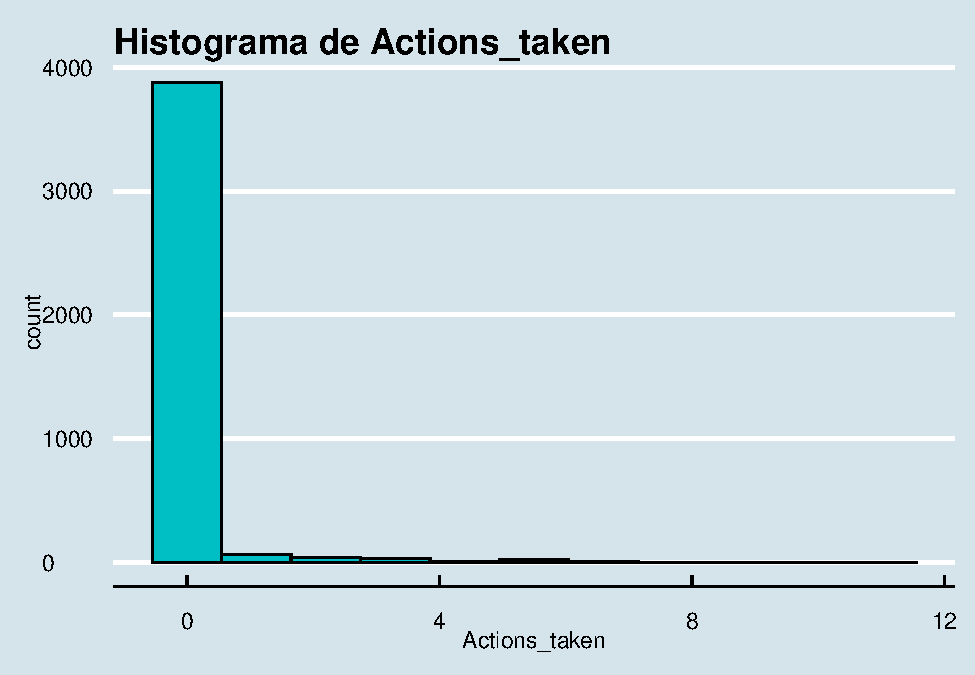
\includegraphics[width=0.5\linewidth]{anacalt-regresion_files/figure-latex/hist_at-1} 

}

\caption{Histograma de Actions taken}\label{fig:hist_at}
\end{figure}

Llama la atención el gran pico en 0, podríamos pensar que son valores
perdidos, pero no podemos asegurarlo ya que es plausible que se hayan
tomado 0 acciones.

Estudiamos también los cuantiles con un boxplot (Figura
\ref{fig:box_at}). Donde vemos que el 75\% de los valores son 0, solo
algunos valores son outliers.

\begin{verbatim}
##   0%  25%  50%  75% 100% 
##    0    0    0    0   11
\end{verbatim}

\begin{figure}

{\centering 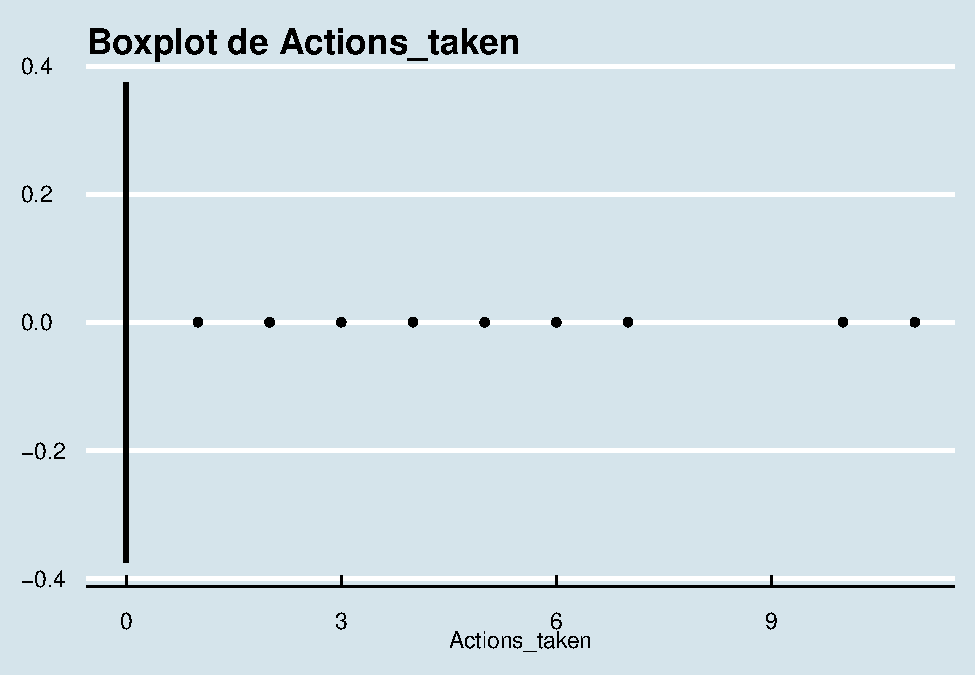
\includegraphics[width=0.5\linewidth]{anacalt-regresion_files/figure-latex/box_at-1} 

}

\caption{Boxplot de Actions taken}\label{fig:box_at}
\end{figure}

Estudiamos la forma de la variable Actions\_taken. Para ello miramos la
media, sd, skewness y kurtosis.

\begin{verbatim}
## [1] "Media: 0.1088"
\end{verbatim}

\begin{verbatim}
## [1] "Deviación estándar: 0.6446"
\end{verbatim}

Para estudiar la skewness y la kurtosis usaremos los tests de D'Agostino
y Anscombe respectivamente.

\begin{verbatim}
## [1] "Skewness: 7.9659"
\end{verbatim}

\begin{verbatim}
## 
##  D'Agostino skewness test
## 
## data:  anacalt$Actions_taken
## skew = 7.9659, z = 63.3294, p-value < 2.2e-16
## alternative hypothesis: data have a skewness
\end{verbatim}

Dado que la skewness \textgreater{} 0 la distribución está sesgada a la
derecha. Ademas el valor de p-value del test de D'agostino es menor que
0.05, por lo que podemos afirmar con seguridad que la distribución está
sesgada a la derecha.

\begin{verbatim}
## [1] "Kurtosis: 80.5755"
\end{verbatim}

\begin{verbatim}
## 
##  Anscombe-Glynn kurtosis test
## 
## data:  anacalt$Actions_taken
## kurt = 80.576, z = 39.005, p-value < 2.2e-16
## alternative hypothesis: kurtosis is not equal to 3
\end{verbatim}

Dado que la kurtosis \textgreater{} 0 la distribución tiene colas
pesadas. Además el valor de p-value del test de Anscombe es menor que
0.05, por lo que podemos afirmar con seguridad que la distribución no es
normal. Podemos verlo mejor con un gráfico de densidad en la Figura
\ref{fig:densidad_at}.

\begin{figure}

{\centering 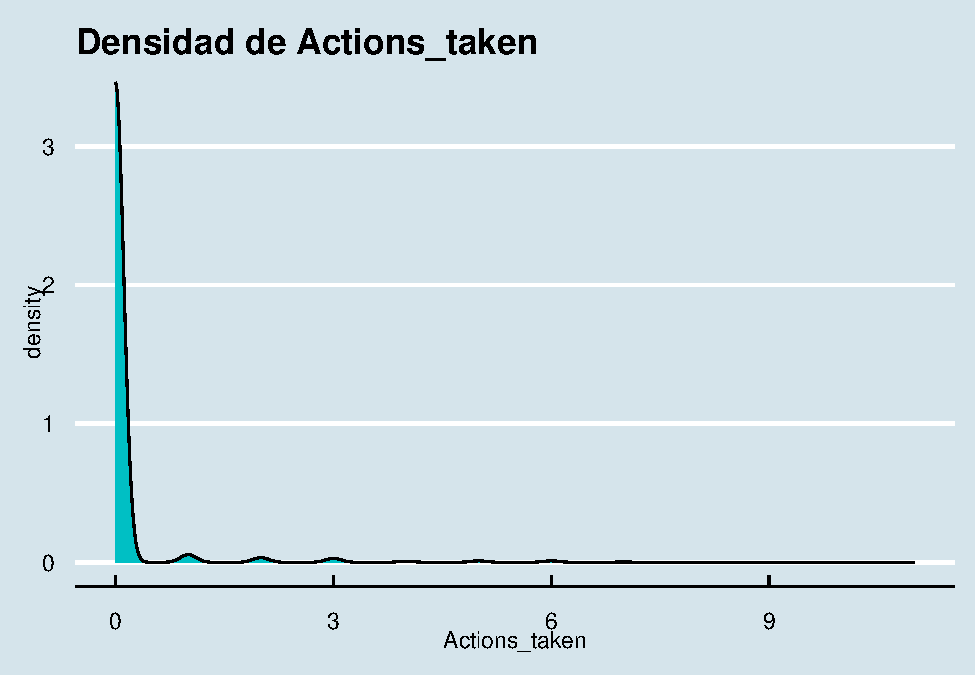
\includegraphics[width=0.5\linewidth]{anacalt-regresion_files/figure-latex/densidad_at-1} 

}

\caption{Densidad de Actions taken}\label{fig:densidad_at}
\end{figure}

Podemos ver como la distribución es significativamente densa en el valor
0 mientras que el resto de valores son muy poco probables.

Estudiamos la normalidad de la variable Actions\_taken con un test de
Shapiro-Wilk y el QQ-plot. Donde vemos que el valor de p-value es menor
que 0.05, por lo que la variable Actions\_taken no sigue una
distribución normal. Lo vemos también el QQ-plot (Figura
\ref{fig:qq_at}).

\begin{verbatim}
## 
##  Shapiro-Wilk normality test
## 
## data:  anacalt$Actions_taken
## W = 0.16301, p-value < 2.2e-16
\end{verbatim}

\begin{figure}

{\centering 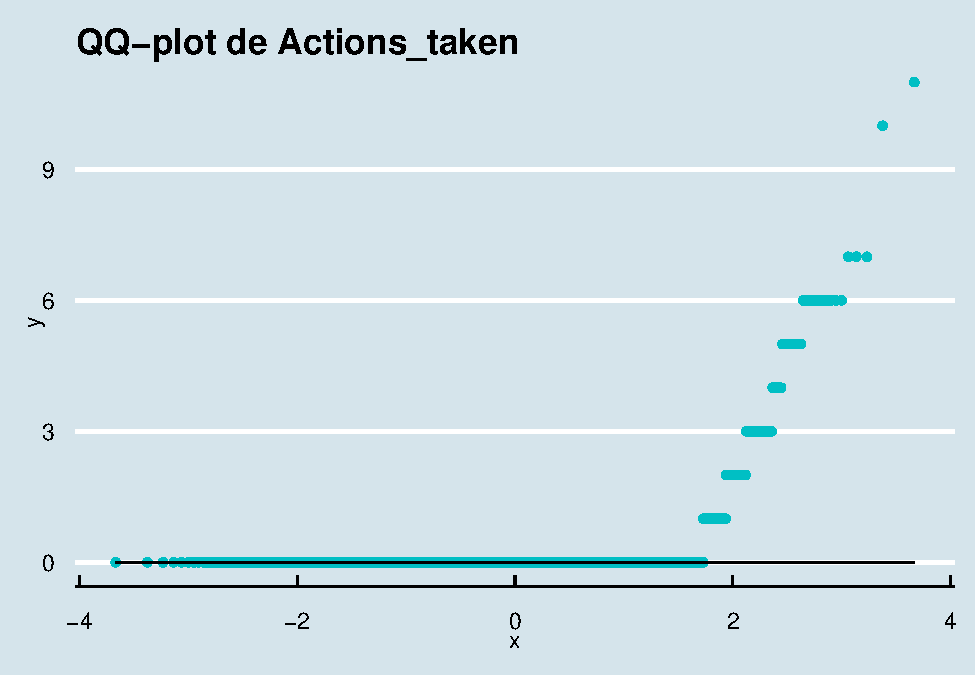
\includegraphics[width=0.5\linewidth]{anacalt-regresion_files/figure-latex/qq_at-1} 

}

\caption{QQ-plot de Actions taken}\label{fig:qq_at}
\end{figure}

\hypertarget{variables-booleanas}{%
\subsubsection{Variables booleanas}\label{variables-booleanas}}

Estudiamos la variable `Liberal', `Unconstitutional',
`Precedent\_alteration', `Unanimous' y `Lower\_court\_disagreement' las
cuales son variables booleanas de valores entre 0 y 1. Por lo que parece
que son variables categóricas binarias. Transformamos las variables a
factor con valores `No' y `Yes' y visualizamos las variables en barplots
(Figura \ref{fig:bar_bool}).

\begin{itemize}
\tightlist
\item
  Para la variable `Liberal' vemos que la mayoría de los valores son
  `Yes' pero no hay una gran diferencia.
\item
  Para la variable `Unconstitutional' vemos que la mayoría de los
  valores son `No' y con una gran diferencia en relación a los `Yes'.
\item
  Para la variable `Precedent\_alteration' vemos que la mayoría de los
  valores son `No' y con una gran diferencia en relación a los `Yes'.
\item
  Para la variable `Unanimous' vemos que la mayoría de los valores son
  `No' y con un diferencia significativa en relación a los `Yes'.
\item
  Para la variable `Lower\_court\_disagreement' vemos que la mayoría de
  los valores son `No' y con un diferencia significativa en relación a
  los `Yes'.
\end{itemize}

\begin{figure}

{\centering 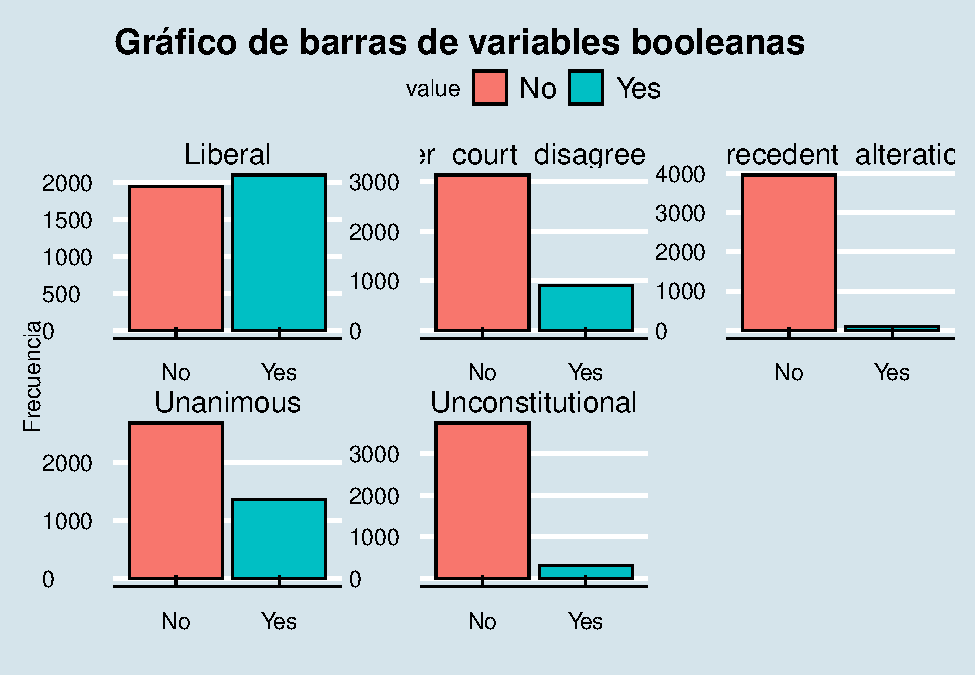
\includegraphics[width=1\linewidth]{anacalt-regresion_files/figure-latex/bar_bool-1} 

}

\caption{ Gráficos de barras de las variables booleanas}\label{fig:bar_bool}
\end{figure}

\hypertarget{variable-year_of_decision}{%
\subsubsection{Variable
`Year\_of\_decision'}\label{variable-year_of_decision}}

Estudiamos la variable `Year\_of\_decision'. Sabemos que pertenece al
rango {[}1953-1988{]}. Para más detalle, vemos un histograma en la
Figura (\ref{fig:hist_year}).

\begin{figure}

{\centering 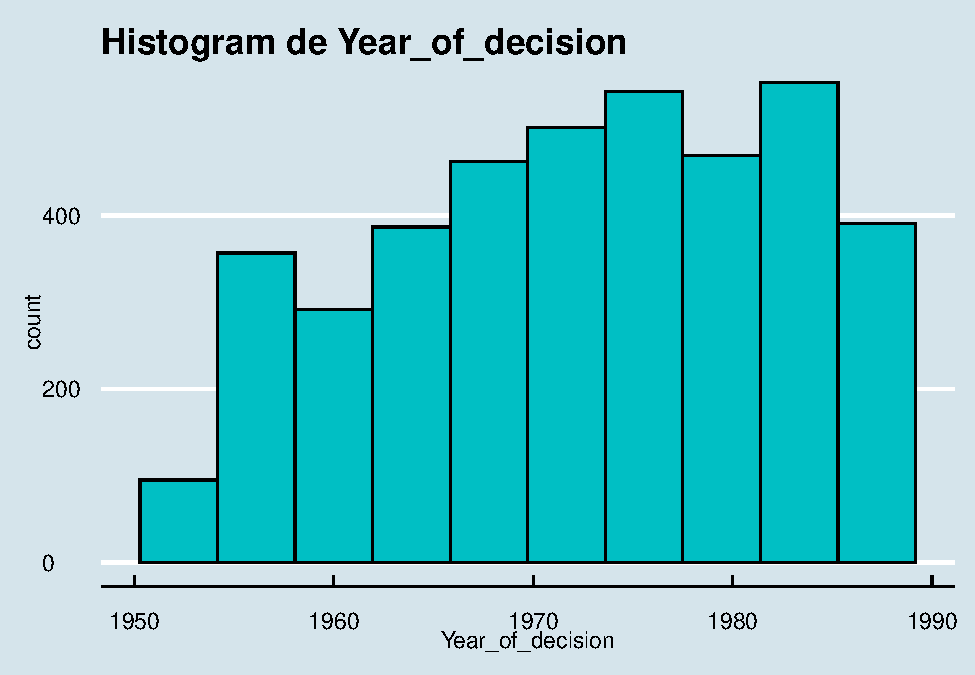
\includegraphics[width=0.5\linewidth]{anacalt-regresion_files/figure-latex/hist_year-1} 

}

\caption{Histograma de Year of decision}\label{fig:hist_year}
\end{figure}

Estudiamos también los cuantiles con un boxplot (Figura
\ref{fig:box_year}). Donde vemos que los valores parecen estar bastante
repartidos con algo de mayor frecuencia hacia el rango superior.

\begin{verbatim}
##   0%  25%  50%  75% 100% 
## 1953 1964 1973 1981 1988
\end{verbatim}

\begin{figure}

{\centering 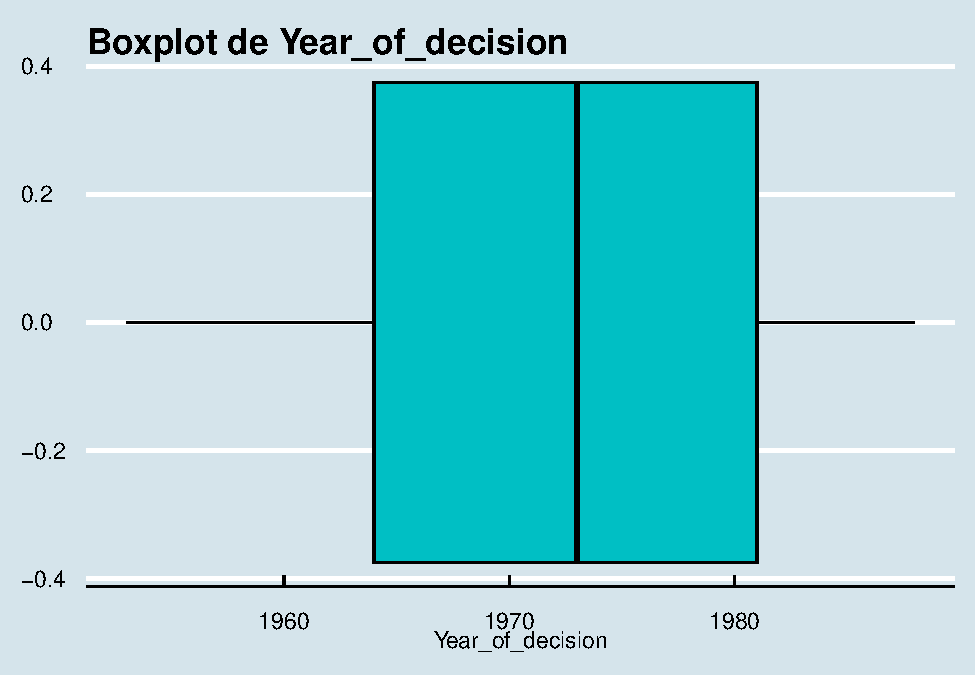
\includegraphics[width=0.5\linewidth]{anacalt-regresion_files/figure-latex/box_year-1} 

}

\caption{Boxplot de Year of decision}\label{fig:box_year}
\end{figure}

Estudiamos para más detalle la forma de la variable. Usamos la media,
sd, skewness y kurtosis.

\begin{verbatim}
## [1] "Media: 1972.3485"
\end{verbatim}

\begin{verbatim}
## [1] "Deviación estándar: 9.851"
\end{verbatim}

Para estudiar la skewness y la kurtosis usaremos los tests de D'Agostino
y Anscombe respectivamente.

\begin{verbatim}
## [1] "Skewness: -0.1706"
\end{verbatim}

\begin{verbatim}
## 
##  D'Agostino skewness test
## 
## data:  anacalt$Year_of_decision
## skew = -0.17057, z = -4.40935, p-value = 1.037e-05
## alternative hypothesis: data have a skewness
\end{verbatim}

Dados que skewness \textless{} 0 la distribución está sesgada a la
izquierda Además el valor de p-value del test de D'agostino es menor que
0.05, por lo que podemos afirmar con seguridad que la distribución está
sesgada.

\begin{verbatim}
## [1] "Kurtosis: 1.8948"
\end{verbatim}

\begin{verbatim}
## 
##  Anscombe-Glynn kurtosis test
## 
## data:  anacalt$Year_of_decision
## kurt = 1.8948, z = -41.0356, p-value < 2.2e-16
## alternative hypothesis: kurtosis is not equal to 3
\end{verbatim}

Dado que kurtosis \textgreater{} 0 la distribución tiene colas pesadas.
Además el valor de p-value del test de Anscombe es menor que 0.05, por
lo que podemos afirmar con seguridad que la distribución tiene colas
pesadas. Podemos verlo mejor con un gráfico de densidad
\ref{fig:densidad_year}.

\begin{figure}

{\centering 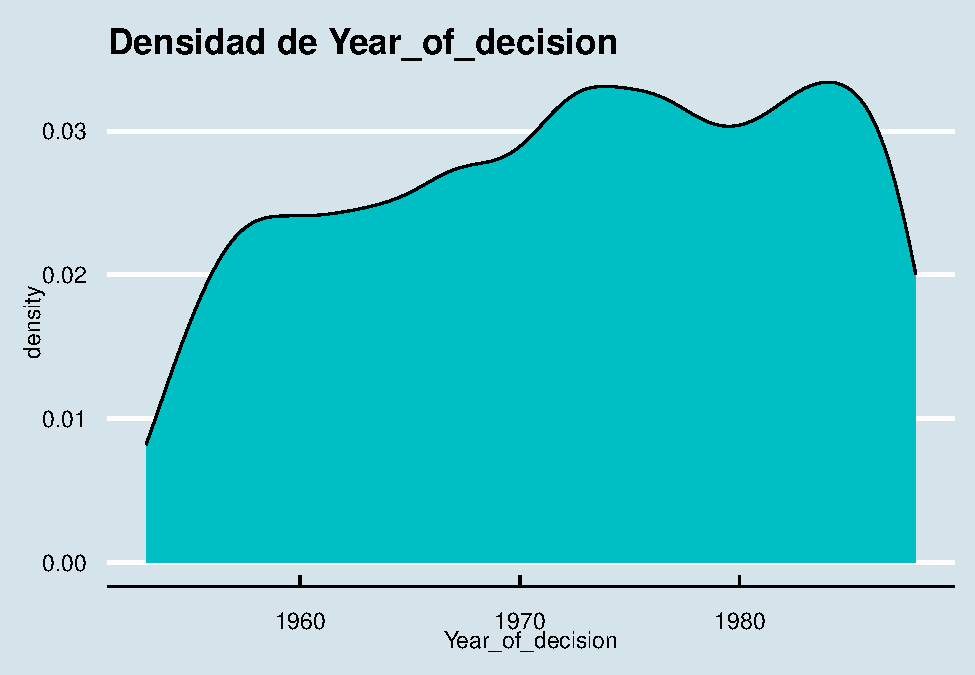
\includegraphics[width=0.5\linewidth]{anacalt-regresion_files/figure-latex/densidad_year-1} 

}

\caption{Densidad de Year of decision}\label{fig:densidad_year}
\end{figure}

Estudiamos la normalidad de la variable Year\_of\_decision con un test
de Shapiro-Wilk y el QQ-plot. Donde vemos que el valor de p-value es
menor que 0.05, por lo que la variable Year\_of\_decision no sigue una
distribución normal. Lo vemos también el QQ-plot (Figura
\ref{fig:qq_year}) donde podemos ver como tiene una forma de `S' muy
aplastada, por lo que no es normal.

\begin{verbatim}
## 
##  Shapiro-Wilk normality test
## 
## data:  anacalt$Year_of_decision
## W = 0.95709, p-value < 2.2e-16
\end{verbatim}

\begin{figure}

{\centering 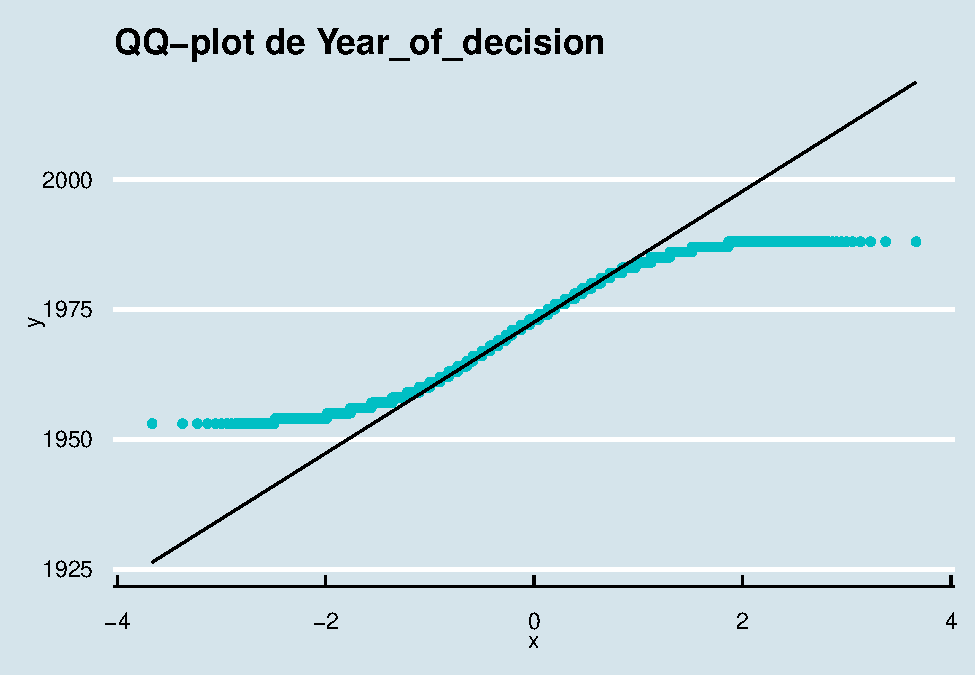
\includegraphics[width=0.5\linewidth]{anacalt-regresion_files/figure-latex/qq_year-1} 

}

\caption{QQ-plot de Year of decision}\label{fig:qq_year}
\end{figure}

\hypertarget{variable-de-output-log_exposure}{%
\subsubsection{Variable de output
``Log\_exposure''}\label{variable-de-output-log_exposure}}

Estudiamos ahora la variable de output ``Log\_exposure''. Sabemos que
pertenece al rango {[}0-2.3{]}. Por lo que es una variable continua.
Para más detalle, vemos un histograma en la Figura (\ref{fig:hist_log}).
Donde vemos que hay un pequeño detalle en el valor 0 y a partir de 0.5
va creciendo casi de manera exponencial.

\begin{figure}

{\centering 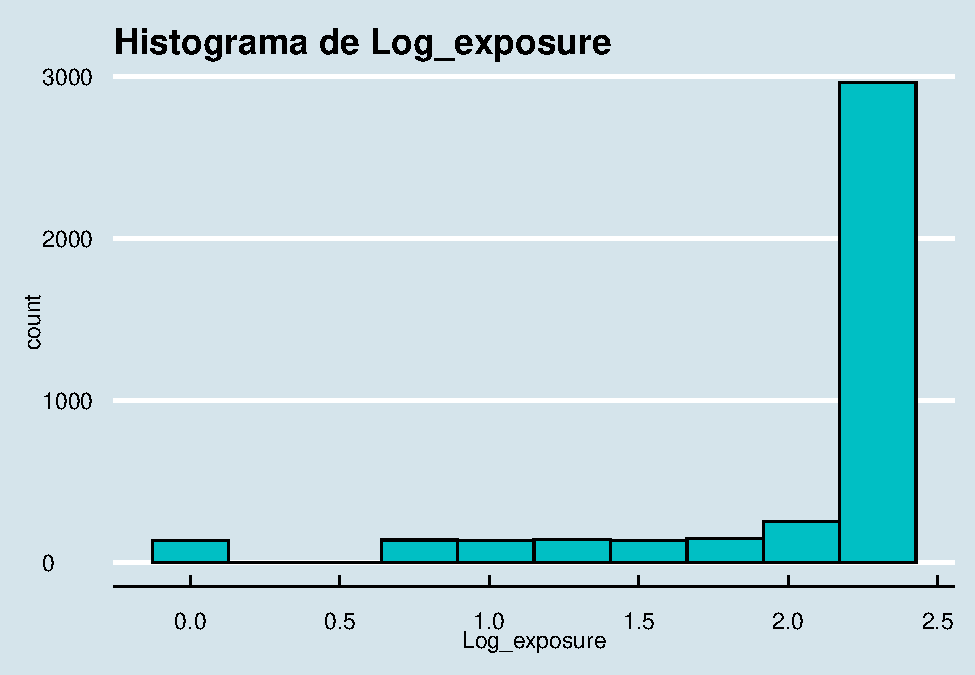
\includegraphics[width=0.5\linewidth]{anacalt-regresion_files/figure-latex/hist_log-1} 

}

\caption{Histograma de Log exposure}\label{fig:hist_log}
\end{figure}

Estudiaremos también los cuantiles con un boxplot (Figura
\ref{fig:box_log}). Donde vemos que el 50\% de los valores superiores es
exactamente 2.3, esto se visualiza perfectamente en el boxplot.

\begin{verbatim}
##   0%  25%  50%  75% 100% 
## 0.00 2.08 2.30 2.30 2.30
\end{verbatim}

\begin{figure}

{\centering 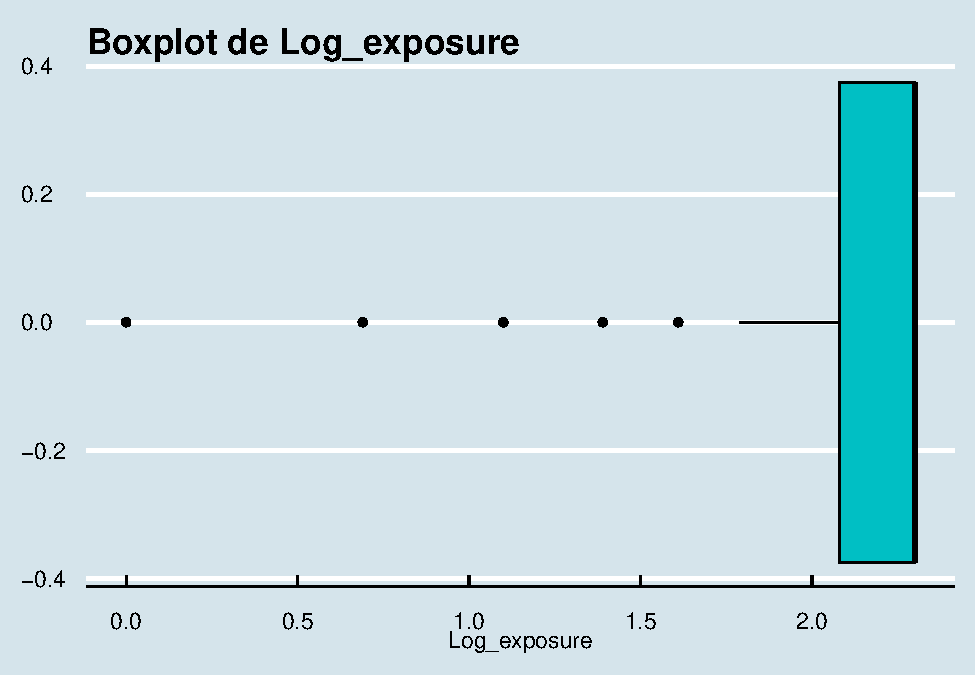
\includegraphics[width=0.5\linewidth]{anacalt-regresion_files/figure-latex/box_log-1} 

}

\caption{Boxplot de Log exposure}\label{fig:box_log}
\end{figure}

Estudiamos para más detalle la forma de la variable. Usamos la media,
sd, skewness y kurtosis.

\begin{verbatim}
## [1] "Media: 2.0337"
\end{verbatim}

\begin{verbatim}
## [1] "Deviación estándar: 0.5495"
\end{verbatim}

Para estudiar la skewness y la kurtosis usaremos los tests de D'Agostino
y Anscombe respectivamente.

\begin{verbatim}
## [1] "Skewness: -2.3454"
\end{verbatim}

\begin{verbatim}
## 
##  D'Agostino skewness test
## 
## data:  anacalt$Log_exposure
## skew = -2.3454, z = -37.8307, p-value < 2.2e-16
## alternative hypothesis: data have a skewness
\end{verbatim}

Dado que skewness \textless{} 0 la distribución está sesgada a la
izquierda Además el valor de p-value del test de D'agostino es menor que
0.05, por lo que podemos afirmar con seguridad que la distribución está
sesgada.

\begin{verbatim}
## [1] "Kurtosis: 7.8682"
\end{verbatim}

\begin{verbatim}
## 
##  Anscombe-Glynn kurtosis test
## 
## data:  anacalt$Log_exposure
## kurt = 7.8682, z = 21.0267, p-value < 2.2e-16
## alternative hypothesis: kurtosis is not equal to 3
\end{verbatim}

Dado que kurtosis \textgreater{} 0 la distribución tiene colas pesadas.
Además el valor de p-value del test de Anscombe es menor que 0.05, por
lo que podemos afirmar con seguridad que la distribución tiene colas
pesadas. Podemos verlo mejor con un gráfico de densidad
\ref{fig:densidad_log}.

\begin{figure}

{\centering 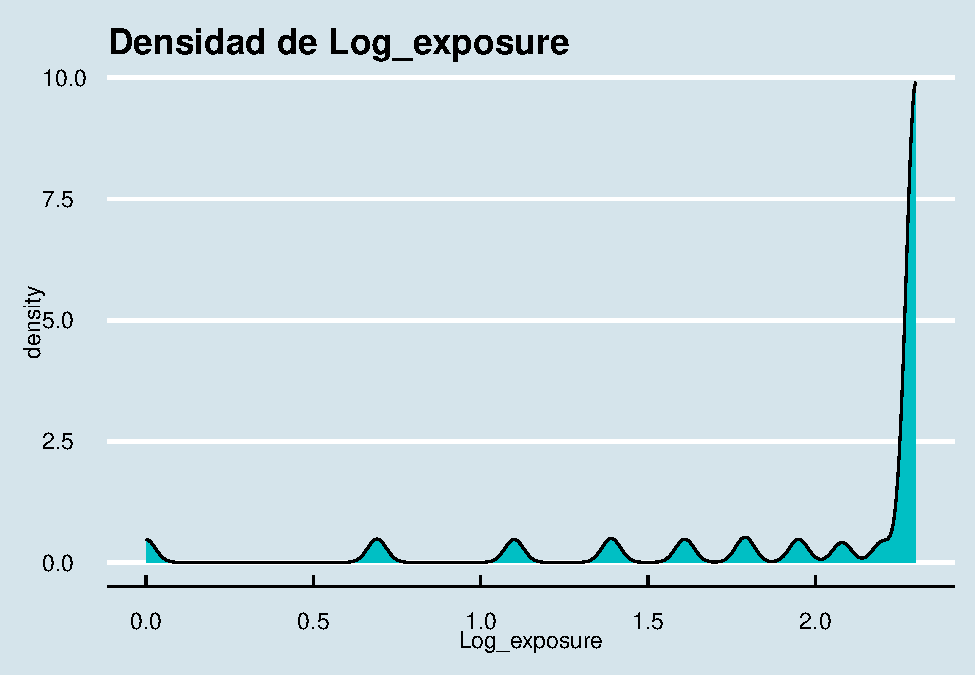
\includegraphics[width=0.5\linewidth]{anacalt-regresion_files/figure-latex/densidad_log-1} 

}

\caption{Densidad de Log exposure}\label{fig:densidad_log}
\end{figure}

Se puede ver como la mayoría de valores se concentran sobre el 2.3.

Estudiamos también la normalidad de la variable Log\_exposure con un
test de Shapiro-Wilk y el QQ-plot. Donde vemos que el valor de p-value
es menor que 0.05, por lo que la variable Log\_exposure no sigue una
distribución normal. Lo vemos también el QQ-plot (Figura
\ref{fig:qq_log}) donde vemos bastante claramente que la variable
Log\_exposure no sigue una distribución normal.

\begin{verbatim}
## 
##  Shapiro-Wilk normality test
## 
## data:  anacalt$Log_exposure
## W = 0.55506, p-value < 2.2e-16
\end{verbatim}

\begin{figure}

{\centering 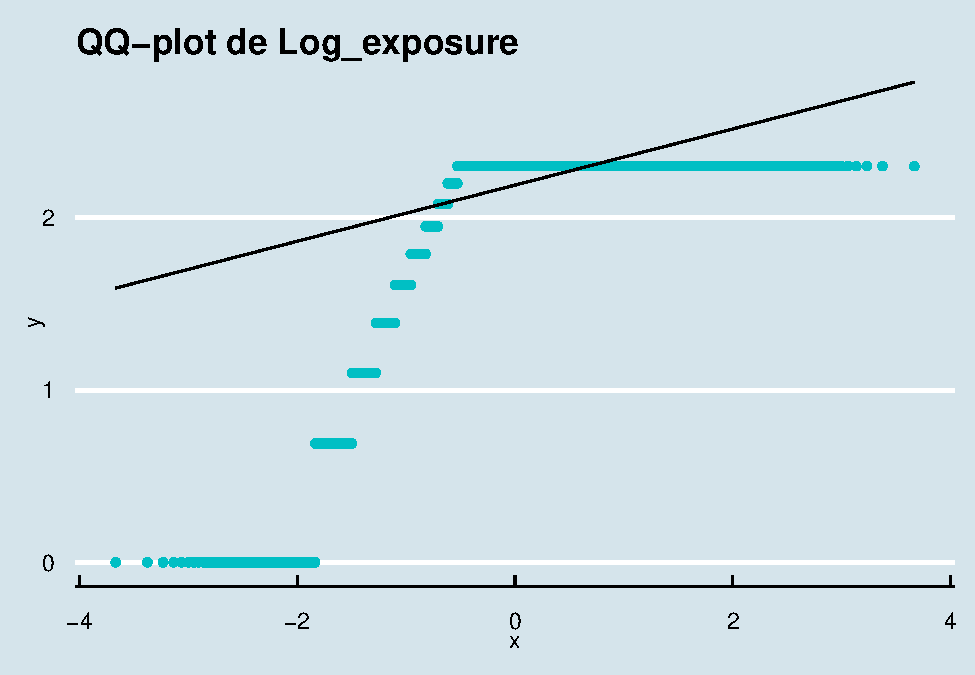
\includegraphics[width=0.5\linewidth]{anacalt-regresion_files/figure-latex/qq_log-1} 

}

\caption{QQ-plot de Log exposure}\label{fig:qq_log}
\end{figure}

\hypertarget{anuxe1lisis-bivariante}{%
\subsection{Análisis bivariante}\label{anuxe1lisis-bivariante}}

Tras el análisis de cada variable por separado, haremos un análisis
bivariable, donde veremos la relación entre las variables.

\hypertarget{correlaciuxf3n-entre-variables-numuxe9ricas}{%
\subsubsection{Correlación entre variables
numéricas}\label{correlaciuxf3n-entre-variables-numuxe9ricas}}

Para ver la correlación entre las variables numéricas usaremos el método
de Spearman pues las variables no siguen una distribución normal (ver
Figura \ref{fig:corr}).

\begin{figure}

{\centering 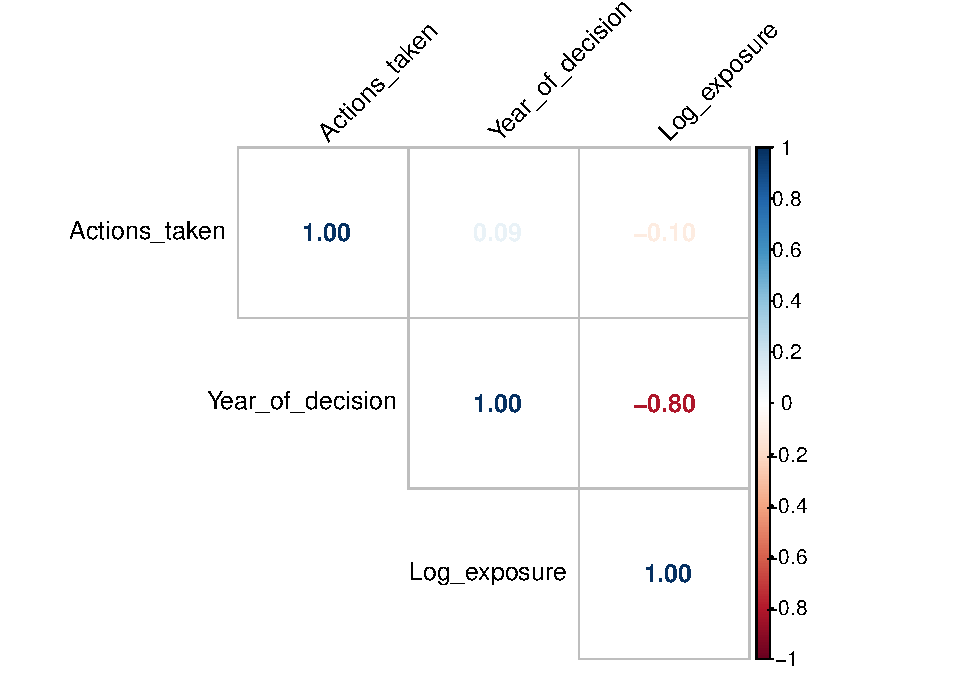
\includegraphics[width=0.75\linewidth]{anacalt-regresion_files/figure-latex/corr-1} 

}

\caption{Correlación entre variables numéricas}\label{fig:corr}
\end{figure}

Podemos observar como la variable de input `Year\_of\_decision' tiene
una correlación negativa con la variable de output `Log\_exposure', lo
que indica que a mayor año de decisión, menor es el valor de
`Log\_exposure'. Podemos verlo mejor con un scatterplot (Figura
\ref{fig:sc_year_log}).

\begin{figure}

{\centering 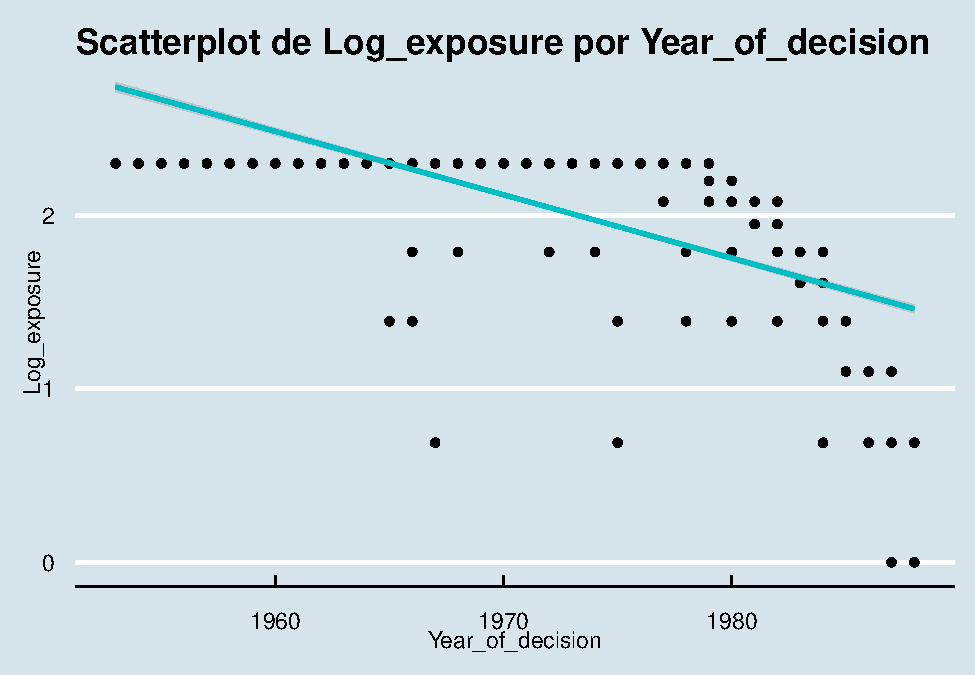
\includegraphics[width=0.5\linewidth]{anacalt-regresion_files/figure-latex/sc_year_log-1} 

}

\caption{Scatterplot de Log exposure por Year of decision}\label{fig:sc_year_log}
\end{figure}

Podemos observar como los valores previos a 1960 son prácticamente todos
2.3 y a partir de 1960 se empiezan a descender hasta 0. Por lo tanto la
relación entre ambas variables es negativa y podemos verlo de mejor
manera con una media por años.

\begin{figure}

{\centering 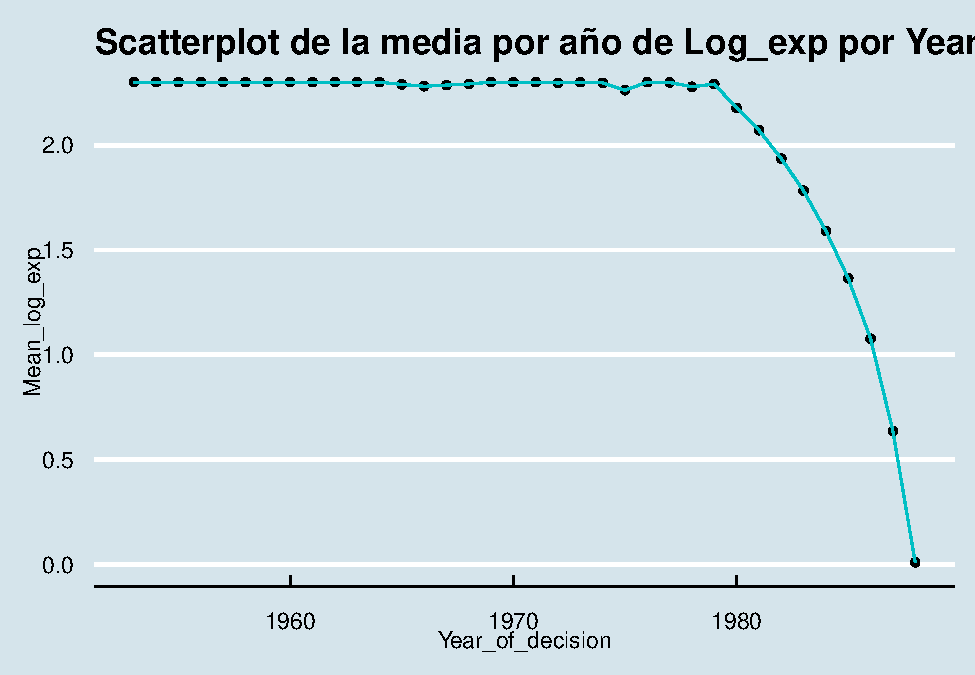
\includegraphics[width=0.5\linewidth]{anacalt-regresion_files/figure-latex/unnamed-chunk-22-1} 

}

\caption{Scatterplot de la media por año de Log exp por Year of decision}\label{fig:unnamed-chunk-22}
\end{figure}

Podemos observar como la media de Log\_exposure se mantiene sobre 2.3
hasta finales de los 70 y va claramente descendiendo a medida que
aumenta el año de decisión.

\hypertarget{relaciuxf3n-entre-variables-categuxf3ricas}{%
\subsubsection{Relación entre variables
categóricas}\label{relaciuxf3n-entre-variables-categuxf3ricas}}

Para ver la relación entre las variables categóricas usaremos tablas de
contingencia y gráficos de mosaico. Primero vemos una tabla de
contingencia que compara cada variable en las Figuras
\ref{fig:cat_grid1} y \ref{fig:cat_grid2}.

\begin{figure}

{\centering 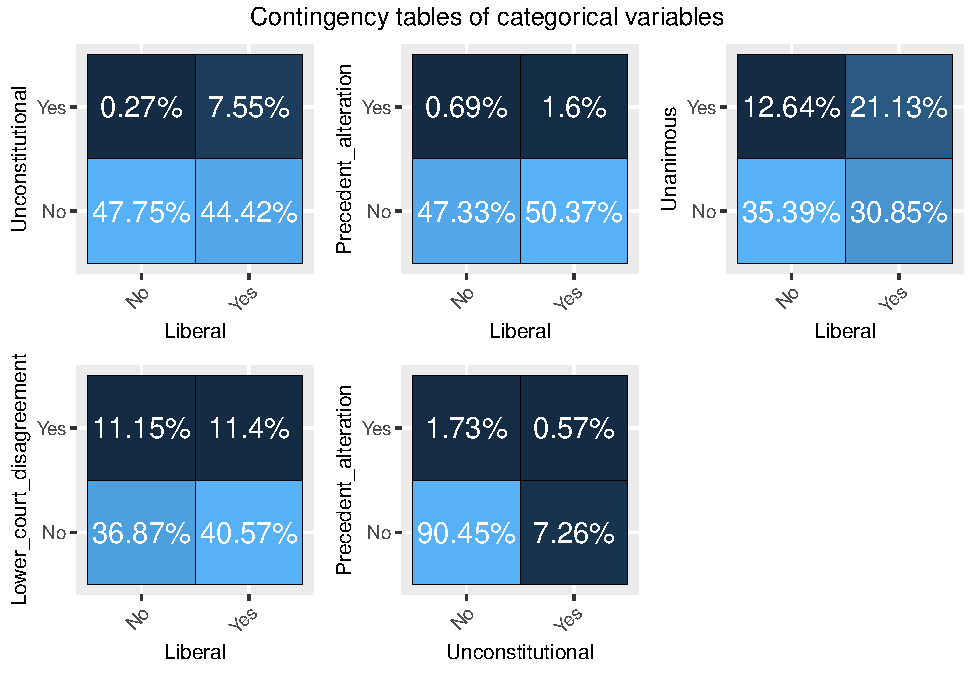
\includegraphics[width=0.75\linewidth]{anacalt-regresion_files/figure-latex/cat_grid1-1} 

}

\caption{Tablas de contingencia de las variables categóricas (1)}\label{fig:cat_grid1}
\end{figure}
\begin{figure}

{\centering 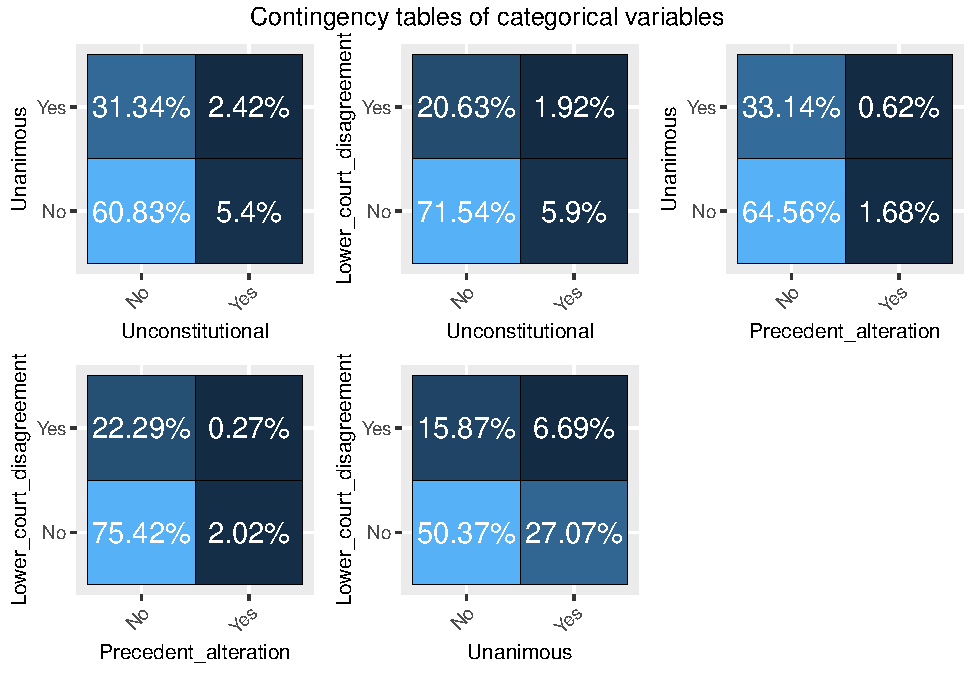
\includegraphics[width=0.75\linewidth]{anacalt-regresion_files/figure-latex/cat_grid2-1} 

}

\caption{Tablas de contingencia de las variables categóricas (2)}\label{fig:cat_grid2}
\end{figure}

Observarndo las tablas de contingencia podemos ver como algunas
variables tienen una relación clara. Resalta que el 90\% de los casos
son `No'`Unconstitutional' y `No' `Precedent\_alteration', por lo que
parece que no hay casos inconstitucionales sin que haya una ``alteración
precedente''. Además vemos que el 75\% de los casos son `NO'
`Precedent\_alteration' y `No' `Lower\_court\_disagreement', por lo que
parece que no hay muchos casos de alteración precedente sin que haya un
desacuerdo de la corte inferior. Por último, vemos que el 71\% de los
casos son `No' `Lower\_court\_disagreement' y `No' `Unconstitutional',
por lo que parece que no hay muchos casos de desacuerdo de la corte
inferior sin que haya un caso inconstitucional.

\hypertarget{relaciuxf3n-con-la-variable-de-output}{%
\subsubsection{Relación con la variable de
output}\label{relaciuxf3n-con-la-variable-de-output}}

Analizaremos la relación de las variables con la variable de output.
Para ello, usaremos boxplots (Figura \ref{fig:grid_box}) para las
variables categóricas y scatterplots (Figura \ref{fig:grid_sca}) para
las variables numéricas.

\begin{figure}

{\centering 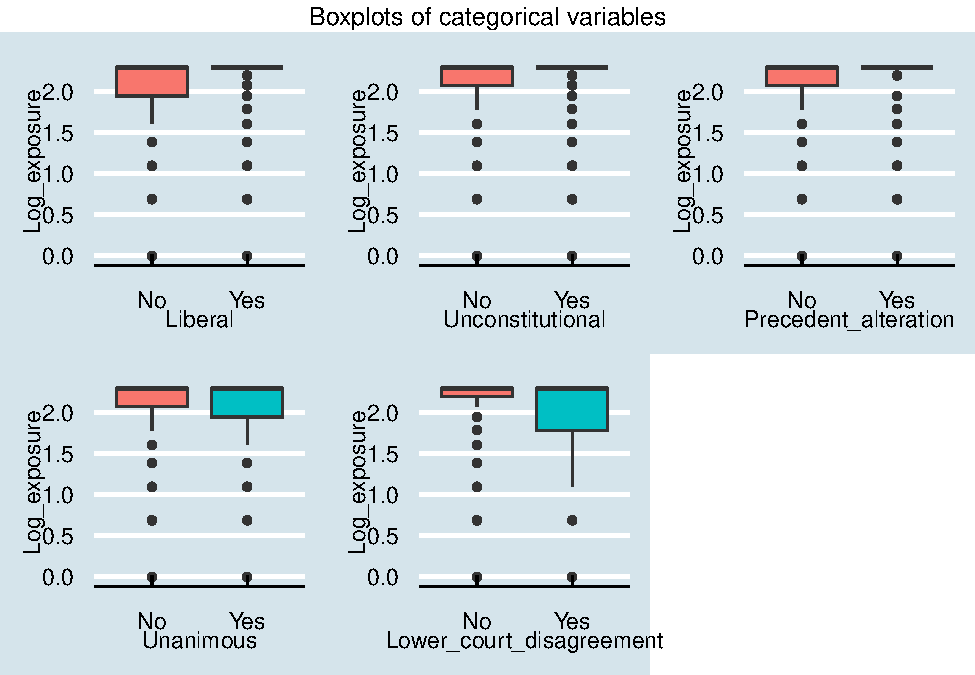
\includegraphics[width=0.75\linewidth]{anacalt-regresion_files/figure-latex/grid_box-1} 

}

\caption{Boxplots de las variables categóricas}\label{fig:grid_box}
\end{figure}

\begin{figure}

{\centering 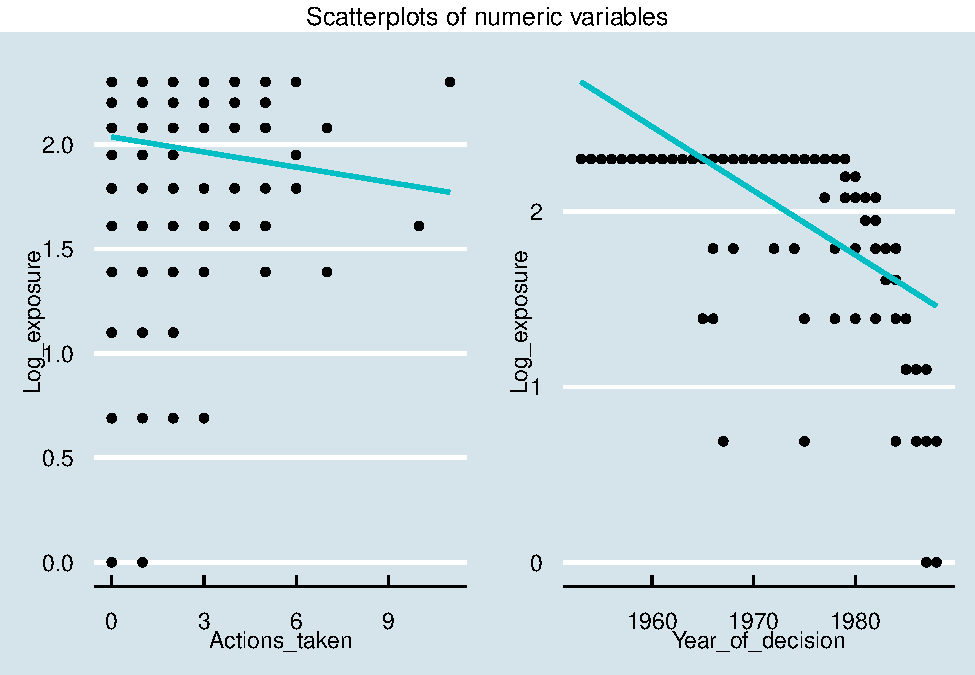
\includegraphics[width=0.75\linewidth]{anacalt-regresion_files/figure-latex/grid_sca-1} 

}

\caption{Scatterplots de las variables numéricas}\label{fig:grid_sca}
\end{figure}

Al igual que lo estudiado en el apartado de correlación, vemos en la
Figura \ref{fig:grid_sca} que Year\_of\_decisión parece tener una
relación cuadrática con Log\_exposure.

\hypertarget{modelo-de-regresiuxf3n}{%
\section{Modelo de regresión}\label{modelo-de-regresiuxf3n}}

\hypertarget{metodologuxeda-de-trabajo}{%
\subsection{Metodología de trabajo}\label{metodologuxeda-de-trabajo}}

Para la realización del modelo de regresión lineal, he decidido usar la
técnica de backward elimination. Esta técnica consiste en ir eliminando
variables del modelo hasta que todas las variables que quedan son
significativas. Una vez se consiga un modelo satisfactorio a este nivel,
se estudiará la posibilidad de añadir interacciones entre variables. Y
tras esto se estudiará la posibilidad de añadir variables polinómicas.

\hypertarget{preparaciuxf3n-del-dataset}{%
\subsection{Preparación del dataset}\label{preparaciuxf3n-del-dataset}}

Dado que el modelo de regresión lineal necesita de variables numéricas,
vamos a convertir las variables categóricas en numéricas. Como son
variables binarias, convertimos los valores `Yes' en 1 y los valores
`No' en 0.

\begin{verbatim}
##  Actions_taken        Liberal       Unconstitutional  Precedent_alteration
##  Min.   : 0.0000   Min.   :0.0000   Min.   :0.00000   Min.   :0.00000     
##  1st Qu.: 0.0000   1st Qu.:0.0000   1st Qu.:0.00000   1st Qu.:0.00000     
##  Median : 0.0000   Median :1.0000   Median :0.00000   Median :0.00000     
##  Mean   : 0.1088   Mean   :0.5197   Mean   :0.07823   Mean   :0.02295     
##  3rd Qu.: 0.0000   3rd Qu.:1.0000   3rd Qu.:0.00000   3rd Qu.:0.00000     
##  Max.   :11.0000   Max.   :1.0000   Max.   :1.00000   Max.   :1.00000     
##    Unanimous      Year_of_decision Lower_court_disagreement  Log_exposure  
##  Min.   :0.0000   Min.   :1953     Min.   :0.0000           Min.   :0.000  
##  1st Qu.:0.0000   1st Qu.:1964     1st Qu.:0.0000           1st Qu.:2.080  
##  Median :0.0000   Median :1973     Median :0.0000           Median :2.300  
##  Mean   :0.3376   Mean   :1972     Mean   :0.2256           Mean   :2.034  
##  3rd Qu.:1.0000   3rd Qu.:1981     3rd Qu.:0.0000           3rd Qu.:2.300  
##  Max.   :1.0000   Max.   :1988     Max.   :1.0000           Max.   :2.300
\end{verbatim}

Además, normalizamos los datos y separmos el conjunto de datos en train
y test (80\% y 20\% respectivamente).

\begin{Shaded}
\begin{Highlighting}[]
\NormalTok{test\_size }\OtherTok{\textless{}{-}} \FloatTok{0.2}
\NormalTok{train\_size }\OtherTok{\textless{}{-}} \DecValTok{1} \SpecialCharTok{{-}}\NormalTok{ test\_size}

\FunctionTok{set.seed}\NormalTok{(}\DecValTok{123}\NormalTok{)}

\CommentTok{\# Normalizamos los datos}
\NormalTok{pObj }\OtherTok{\textless{}{-}} \FunctionTok{preProcess}\NormalTok{(num\_anacalt, }\AttributeTok{method=}\FunctionTok{c}\NormalTok{(}\StringTok{\textquotesingle{}range\textquotesingle{}}\NormalTok{))}
\NormalTok{num\_anacalt }\OtherTok{\textless{}{-}} \FunctionTok{predict}\NormalTok{(pObj, num\_anacalt)}

\CommentTok{\# Separamos el conjunto de datos en train y test}
\NormalTok{train\_index }\OtherTok{\textless{}{-}} \FunctionTok{createDataPartition}\NormalTok{(num\_anacalt}\SpecialCharTok{$}\NormalTok{Log\_exposure, }\AttributeTok{p =}\NormalTok{ train\_size, }\AttributeTok{list =} \ConstantTok{FALSE}\NormalTok{)}
\NormalTok{train }\OtherTok{\textless{}{-}}\NormalTok{ num\_anacalt[train\_index, ] }\SpecialCharTok{\%\textgreater{}\%}\NormalTok{ dplyr}\SpecialCharTok{::}\FunctionTok{select}\NormalTok{(}\SpecialCharTok{{-}}\NormalTok{Log\_exposure)}
\NormalTok{test }\OtherTok{\textless{}{-}}\NormalTok{ num\_anacalt[}\SpecialCharTok{{-}}\NormalTok{train\_index, ] }\SpecialCharTok{\%\textgreater{}\%}\NormalTok{ dplyr}\SpecialCharTok{::}\FunctionTok{select}\NormalTok{(}\SpecialCharTok{{-}}\NormalTok{Log\_exposure)}
\NormalTok{train\_lbl }\OtherTok{\textless{}{-}}\NormalTok{ num\_anacalt[train\_index, ]}\SpecialCharTok{$}\NormalTok{Log\_exposure}
\NormalTok{test\_lbl }\OtherTok{\textless{}{-}}\NormalTok{ num\_anacalt[}\SpecialCharTok{{-}}\NormalTok{train\_index, ]}\SpecialCharTok{$}\NormalTok{Log\_exposure}
\end{Highlighting}
\end{Shaded}

\hypertarget{modelo-de-regresiuxf3n-lineal}{%
\subsection{Modelo de regresión
lineal}\label{modelo-de-regresiuxf3n-lineal}}

\hypertarget{modelo-inicial}{%
\subsubsection{Modelo inicial}\label{modelo-inicial}}

Primero, vamos a crear un modelo inicial con todas las variables. Para
ello, usaremos la función lm(). Comenzamos con un modelo inicial con
todas las variables.

\begin{verbatim}
## 
## Call:
## lm(formula = train_lbl ~ ., data = train)
## 
## Residuals:
##      Min       1Q   Median       3Q      Max 
## -0.69106 -0.08625  0.03199  0.13065  0.25765 
## 
## Coefficients:
##                            Estimate Std. Error t value Pr(>|t|)    
## (Intercept)               1.2105886  0.0085834 141.038  < 2e-16 ***
## Actions_taken             0.1279428  0.0539554   2.371   0.0178 *  
## Liberal                  -0.0269254  0.0067701  -3.977 7.13e-05 ***
## Unconstitutional          0.0616941  0.0122485   5.037 4.99e-07 ***
## Precedent_alteration      0.0037307  0.0228494   0.163   0.8703    
## Unanimous                 0.0005367  0.0067669   0.079   0.9368    
## Year_of_decision         -0.5687389  0.0115819 -49.106  < 2e-16 ***
## Lower_court_disagreement -0.0188179  0.0075786  -2.483   0.0131 *  
## ---
## Signif. codes:  0 '***' 0.001 '**' 0.01 '*' 0.05 '.' 0.1 ' ' 1
## 
## Residual standard error: 0.1796 on 3235 degrees of freedom
## Multiple R-squared:  0.4387, Adjusted R-squared:  0.4375 
## F-statistic: 361.2 on 7 and 3235 DF,  p-value: < 2.2e-16
\end{verbatim}

Vemos que el modelo inicial tiene un R\^{}2 de 0.438 y que la variable
`Unanimous' no es significativa. Por lo que la eliminamos, tras esto el
modelo mantiene un R\^{}2 ajustado de 0.438 y la variable
`Precedent\_alterations' no se marca como significativa. Por lo que la
eliminamos también.

\begin{verbatim}
## 
## Call:
## lm(formula = train_lbl ~ . - Unanimous - Precedent_alteration, 
##     data = train)
## 
## Residuals:
##      Min       1Q   Median       3Q      Max 
## -0.69134 -0.08647  0.03295  0.13044  0.25740 
## 
## Coefficients:
##                           Estimate Std. Error t value Pr(>|t|)    
## (Intercept)               1.210791   0.008402 144.100  < 2e-16 ***
## Actions_taken             0.127832   0.053907   2.371   0.0178 *  
## Liberal                  -0.026830   0.006668  -4.024 5.86e-05 ***
## Unconstitutional          0.061857   0.012150   5.091 3.76e-07 ***
## Year_of_decision         -0.568723   0.011573 -49.142  < 2e-16 ***
## Lower_court_disagreement -0.018885   0.007563  -2.497   0.0126 *  
## ---
## Signif. codes:  0 '***' 0.001 '**' 0.01 '*' 0.05 '.' 0.1 ' ' 1
## 
## Residual standard error: 0.1796 on 3237 degrees of freedom
## Multiple R-squared:  0.4387, Adjusted R-squared:  0.4379 
## F-statistic:   506 on 5 and 3237 DF,  p-value: < 2.2e-16
\end{verbatim}

Tras quitar estas 2 variables vemos que el modelo se mantiene en un
R\^{}2 de 0.438 y que la variable `Actions\_taken' es la menos
significativa, por lo que probamos a eliminarla. Por lo que vamos a
eliminarla del modelo pero esto empeora el R\^{}2 ajustado a 0.437, por
lo que la dejamos en el modelo. Observamos como se ajusta este modelo a
los datos en la Figura \ref{fig:model_1}. Calculamos también el MSE
(Mean Squared Error) con el conjunto de test.

\begin{verbatim}
## [1] "MSE: 0.032"
\end{verbatim}

\begin{figure}

{\centering 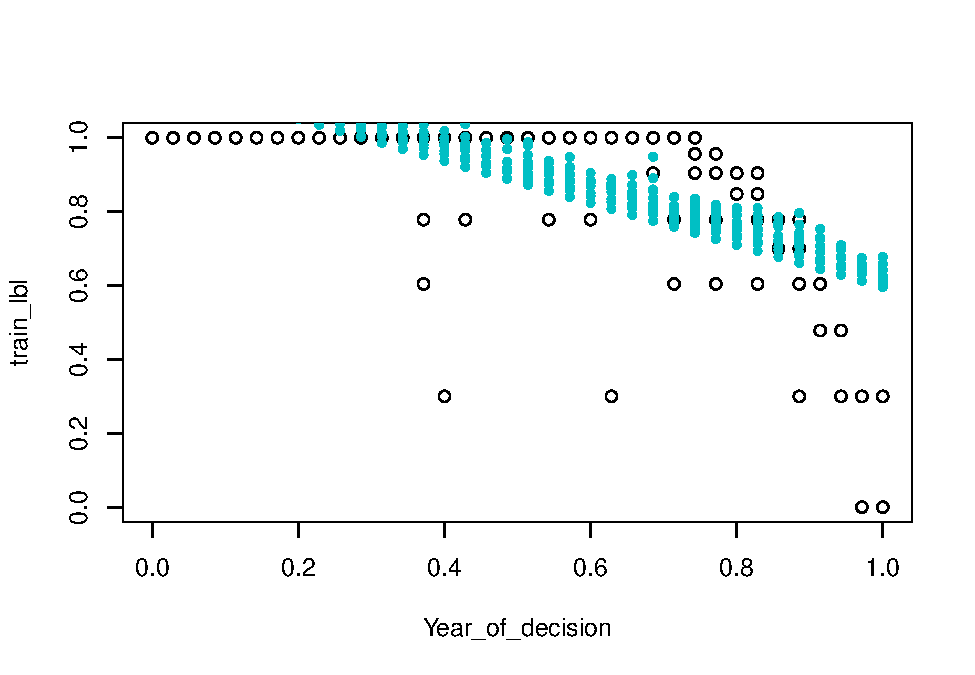
\includegraphics[width=0.75\linewidth]{anacalt-regresion_files/figure-latex/model_1-1} 

}

\caption{Ajuste del modelo inicial}\label{fig:model_1}
\end{figure}

\hypertarget{interacciones}{%
\subsubsection{Interacciones}\label{interacciones}}

Ahora vamos a estudiar la posibilidad de añadir interacciones entre
variables. Para esto, nos remitimos a la correlación estudiada
anteriormente, y vemos que las variables no parecen tener casi ninguna
correlación entre ellas. Por lo que vamos a probar a añadir
interacciones entre todas las variables e ir podando las menos
significativas.

\begin{verbatim}
## [1] "R^2 ajustado: 0.4451"
\end{verbatim}

Se puede observar como el R\^{}2 ajustado ha pasado de 0.438 a 0.4451.
Por lo que el modelo con las interacciones promete, pero eliminaremos
las variables que no son significativas, o sea la interacción a 4 bandas
y probamos solo con las interacciones a 3 niveles.

\begin{verbatim}
## [1] "R^2 ajustado: 0.4453"
\end{verbatim}

\begin{verbatim}
##                                                                Estimate
## (Intercept)                                                 1.222227152
## Actions_taken                                              -0.424696336
## Unconstitutional                                            0.097722195
## Year_of_decision                                           -0.587533673
## Liberal                                                    -0.074078764
## Lower_court_disagreement                                    0.077502654
## Actions_taken:Unconstitutional                             -1.884254283
## Actions_taken:Year_of_decision                              0.755180790
## Unconstitutional:Year_of_decision                          -0.005863182
## Unconstitutional:Liberal                                   -0.048060108
## Year_of_decision:Liberal                                    0.095116855
## Actions_taken:Liberal                                      -0.042882875
## Actions_taken:Lower_court_disagreement                      2.331755870
## Liberal:Lower_court_disagreement                           -0.026274525
## Unconstitutional:Lower_court_disagreement                   0.155219155
## Year_of_decision:Lower_court_disagreement                  -0.147042930
## Actions_taken:Unconstitutional:Year_of_decision             4.184823226
## Unconstitutional:Year_of_decision:Liberal                   0.013559126
## Actions_taken:Liberal:Lower_court_disagreement             -0.211468828
## Unconstitutional:Liberal:Lower_court_disagreement          -0.083889139
## Actions_taken:Year_of_decision:Lower_court_disagreement    -2.790219053
## Year_of_decision:Liberal:Lower_court_disagreement           0.006733162
## Unconstitutional:Year_of_decision:Lower_court_disagreement -0.105290464
##                                                            Std. Error
## (Intercept)                                                0.01252294
## Actions_taken                                              0.25934947
## Unconstitutional                                           0.27026690
## Year_of_decision                                           0.01931272
## Liberal                                                    0.01628697
## Lower_court_disagreement                                   0.02841556
## Actions_taken:Unconstitutional                             4.18542929
## Actions_taken:Year_of_decision                             0.34653312
## Unconstitutional:Year_of_decision                          0.42367882
## Unconstitutional:Liberal                                   0.27259225
## Year_of_decision:Liberal                                   0.02695230
## Actions_taken:Liberal                                      0.12410800
## Actions_taken:Lower_court_disagreement                     0.92111619
## Liberal:Lower_court_disagreement                           0.03666421
## Unconstitutional:Lower_court_disagreement                  0.18605166
## Year_of_decision:Lower_court_disagreement                  0.04054240
## Actions_taken:Unconstitutional:Year_of_decision            7.88027062
## Unconstitutional:Year_of_decision:Liberal                  0.42812659
## Actions_taken:Liberal:Lower_court_disagreement             0.33691317
## Unconstitutional:Liberal:Lower_court_disagreement          0.16402210
## Actions_taken:Year_of_decision:Lower_court_disagreement    1.10497084
## Year_of_decision:Liberal:Lower_court_disagreement          0.05615805
## Unconstitutional:Year_of_decision:Lower_court_disagreement 0.12114873
##                                                                 t value
## (Intercept)                                                 97.59903668
## Actions_taken                                               -1.63754462
## Unconstitutional                                             0.36157663
## Year_of_decision                                           -30.42210996
## Liberal                                                     -4.54834609
## Lower_court_disagreement                                     2.72747225
## Actions_taken:Unconstitutional                              -0.45019379
## Actions_taken:Year_of_decision                               2.17924564
## Unconstitutional:Year_of_decision                           -0.01383874
## Unconstitutional:Liberal                                    -0.17630768
## Year_of_decision:Liberal                                     3.52908150
## Actions_taken:Liberal                                       -0.34552870
## Actions_taken:Lower_court_disagreement                       2.53144597
## Liberal:Lower_court_disagreement                            -0.71662588
## Unconstitutional:Lower_court_disagreement                    0.83427988
## Year_of_decision:Lower_court_disagreement                   -3.62689296
## Actions_taken:Unconstitutional:Year_of_decision              0.53105070
## Unconstitutional:Year_of_decision:Liberal                    0.03167083
## Actions_taken:Liberal:Lower_court_disagreement              -0.62766566
## Unconstitutional:Liberal:Lower_court_disagreement           -0.51145021
## Actions_taken:Year_of_decision:Lower_court_disagreement     -2.52515175
## Year_of_decision:Liberal:Lower_court_disagreement            0.11989665
## Unconstitutional:Year_of_decision:Lower_court_disagreement  -0.86910082
##                                                                 Pr(>|t|)
## (Intercept)                                                 0.000000e+00
## Actions_taken                                               1.016144e-01
## Unconstitutional                                            7.176922e-01
## Year_of_decision                                           6.628540e-179
## Liberal                                                     5.606414e-06
## Lower_court_disagreement                                    6.416775e-03
## Actions_taken:Unconstitutional                              6.526010e-01
## Actions_taken:Year_of_decision                              2.938567e-02
## Unconstitutional:Year_of_decision                           9.889595e-01
## Unconstitutional:Liberal                                    8.600633e-01
## Year_of_decision:Liberal                                    4.228398e-04
## Actions_taken:Liberal                                       7.297195e-01
## Actions_taken:Lower_court_disagreement                      1.140653e-02
## Liberal:Lower_court_disagreement                            4.736569e-01
## Unconstitutional:Lower_court_disagreement                   4.041852e-01
## Year_of_decision:Lower_court_disagreement                   2.913007e-04
## Actions_taken:Unconstitutional:Year_of_decision             5.954203e-01
## Unconstitutional:Year_of_decision:Liberal                   9.747365e-01
## Actions_taken:Liberal:Lower_court_disagreement              5.302675e-01
## Unconstitutional:Liberal:Lower_court_disagreement           6.090709e-01
## Actions_taken:Year_of_decision:Lower_court_disagreement     1.161246e-02
## Year_of_decision:Liberal:Lower_court_disagreement           9.045725e-01
## Unconstitutional:Year_of_decision:Lower_court_disagreement  3.848568e-01
\end{verbatim}

Vemos que el R\^{}2 ajustado ha pasado de 0.4451 a 0.4453 y la
interacción entre Actions\_taken, Year\_of\_decision y
Lower\_court\_disagreeement tiene un p-valor aceptable. Por lo que
seguimos puliendo este modelo, eliminando todas las viendo que las
interacciones de 3 variables que no son significativas. Así probamos un
modelo con las interacciones entre 2 variables, mantiendo la interacción
de 3 identificada.

\begin{verbatim}
## 
## Call:
## lm(formula = train_lbl ~ Actions_taken * Year_of_decision * Lower_court_disagreement + 
##     Actions_taken * Unconstitutional + Unconstitutional * Year_of_decision + 
##     Unconstitutional * Liberal + Year_of_decision * Liberal + 
##     Actions_taken * Liberal + Liberal * Lower_court_disagreement + 
##     Unconstitutional * Lower_court_disagreement, data = train)
## 
## Residuals:
##      Min       1Q   Median       3Q      Max 
## -0.70247 -0.08747  0.03472  0.13051  0.27312 
## 
## Coefficients:
##                                                         Estimate Std. Error
## (Intercept)                                              1.22161    0.01185
## Actions_taken                                           -0.41609    0.25823
## Year_of_decision                                        -0.58687    0.01806
## Lower_court_disagreement                                 0.08041    0.02074
## Unconstitutional                                         0.11521    0.06398
## Liberal                                                 -0.07419    0.01471
## Actions_taken:Year_of_decision                           0.76640    0.34572
## Actions_taken:Lower_court_disagreement                   2.04525    0.80142
## Year_of_decision:Lower_court_disagreement               -0.14998    0.02734
## Actions_taken:Unconstitutional                           0.34137    0.46449
## Year_of_decision:Unconstitutional                       -0.01677    0.05274
## Unconstitutional:Liberal                                -0.05301    0.05575
## Year_of_decision:Liberal                                 0.09649    0.02359
## Actions_taken:Liberal                                   -0.07199    0.11528
## Lower_court_disagreement:Liberal                        -0.02527    0.01607
## Lower_court_disagreement:Unconstitutional                0.01452    0.02826
## Actions_taken:Year_of_decision:Lower_court_disagreement -2.50821    1.01169
##                                                         t value Pr(>|t|)    
## (Intercept)                                             103.095  < 2e-16 ***
## Actions_taken                                            -1.611 0.107215    
## Year_of_decision                                        -32.494  < 2e-16 ***
## Lower_court_disagreement                                  3.878 0.000108 ***
## Unconstitutional                                          1.801 0.071828 .  
## Liberal                                                  -5.044 4.82e-07 ***
## Actions_taken:Year_of_decision                            2.217 0.026705 *  
## Actions_taken:Lower_court_disagreement                    2.552 0.010755 *  
## Year_of_decision:Lower_court_disagreement                -5.485 4.44e-08 ***
## Actions_taken:Unconstitutional                            0.735 0.462429    
## Year_of_decision:Unconstitutional                        -0.318 0.750568    
## Unconstitutional:Liberal                                 -0.951 0.341771    
## Year_of_decision:Liberal                                  4.090 4.41e-05 ***
## Actions_taken:Liberal                                    -0.625 0.532323    
## Lower_court_disagreement:Liberal                         -1.572 0.116079    
## Lower_court_disagreement:Unconstitutional                 0.514 0.607414    
## Actions_taken:Year_of_decision:Lower_court_disagreement  -2.479 0.013218 *  
## ---
## Signif. codes:  0 '***' 0.001 '**' 0.01 '*' 0.05 '.' 0.1 ' ' 1
## 
## Residual standard error: 0.1782 on 3226 degrees of freedom
## Multiple R-squared:  0.4488, Adjusted R-squared:  0.4461 
## F-statistic: 164.2 on 16 and 3226 DF,  p-value: < 2.2e-16
\end{verbatim}

Vemos que el R\^{}2 ajustado ha pasado de 0.4453 a 0.4461, Por lo que
seguimos podando, en este caso, eliminamos las interacciones
introducidas que no son significativas. Eso significa que solo se
mantiene Year\_of\_decision*Liberal y la interacción de a 3.

\begin{verbatim}
## 
## Call:
## lm(formula = train_lbl ~ Unconstitutional + Actions_taken * Year_of_decision * 
##     Lower_court_disagreement + Year_of_decision * Liberal, data = train)
## 
## Residuals:
##      Min       1Q   Median       3Q      Max 
## -0.71048 -0.08862  0.03759  0.12735  0.26340 
## 
## Coefficients:
##                                                         Estimate Std. Error
## (Intercept)                                              1.22436    0.01172
## Unconstitutional                                         0.06006    0.01207
## Actions_taken                                           -0.42142    0.25000
## Year_of_decision                                        -0.58618    0.01803
## Lower_court_disagreement                                 0.06325    0.01737
## Liberal                                                 -0.07759    0.01432
## Actions_taken:Year_of_decision                           0.72580    0.34082
## Actions_taken:Lower_court_disagreement                   1.90388    0.78997
## Year_of_decision:Lower_court_disagreement               -0.14095    0.02668
## Year_of_decision:Liberal                                 0.08983    0.02285
## Actions_taken:Year_of_decision:Lower_court_disagreement -2.29843    0.98790
##                                                         t value Pr(>|t|)    
## (Intercept)                                             104.460  < 2e-16 ***
## Unconstitutional                                          4.976 6.84e-07 ***
## Actions_taken                                            -1.686 0.091952 .  
## Year_of_decision                                        -32.509  < 2e-16 ***
## Lower_court_disagreement                                  3.641 0.000276 ***
## Liberal                                                  -5.420 6.41e-08 ***
## Actions_taken:Year_of_decision                            2.130 0.033283 *  
## Actions_taken:Lower_court_disagreement                    2.410 0.016005 *  
## Year_of_decision:Lower_court_disagreement                -5.282 1.36e-07 ***
## Year_of_decision:Liberal                                  3.932 8.59e-05 ***
## Actions_taken:Year_of_decision:Lower_court_disagreement  -2.327 0.020049 *  
## ---
## Signif. codes:  0 '***' 0.001 '**' 0.01 '*' 0.05 '.' 0.1 ' ' 1
## 
## Residual standard error: 0.1782 on 3232 degrees of freedom
## Multiple R-squared:  0.4481, Adjusted R-squared:  0.4464 
## F-statistic: 262.4 on 10 and 3232 DF,  p-value: < 2.2e-16
\end{verbatim}

Vemos que hemos conseguido un R\^{}2 ajustado de 0.4464, mejorándolo. Si
probamos a eliminar la interacción de 3 variables que es la menos
significativa y sustituirla por las interacciones de a 2, vemos que el
R\^{}2 ajustado baja a 0.4456 por lo que lo dejamos con ella. Vemos como
este modelo se ajusta a los datos en la Figura \ref{fig:model_2}.
Calculamos también el MSE (Mean Squared Error) con el conjunto de test.

\begin{verbatim}
## [1] "MSE: 0.0317"
\end{verbatim}

\begin{figure}

{\centering 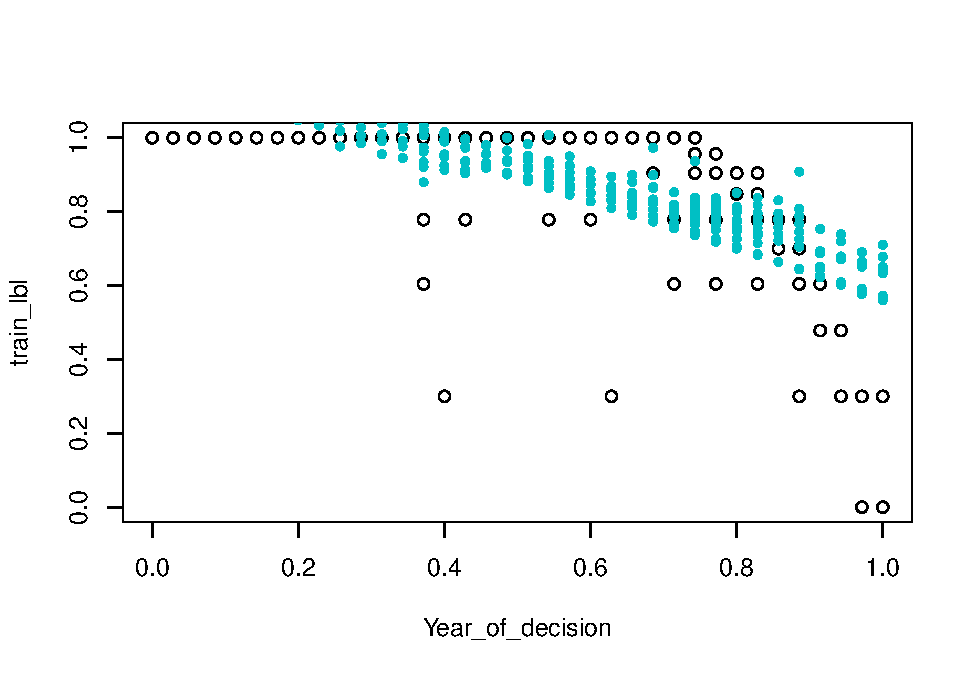
\includegraphics[width=0.75\linewidth]{anacalt-regresion_files/figure-latex/model_2-1} 

}

\caption{Ajuste del modelo con interacciones}\label{fig:model_2}
\end{figure}

\hypertarget{variables-polinuxf3micas}{%
\subsubsection{Variables polinómicas}\label{variables-polinuxf3micas}}

Ahora vamos a estudiar la posibilidad de añadir variables polinómicas.
Para ello, estudiamos las variables en relación con la variable de
output en la Figura \ref{fig:scat_smooth}.

\begin{figure}

{\centering 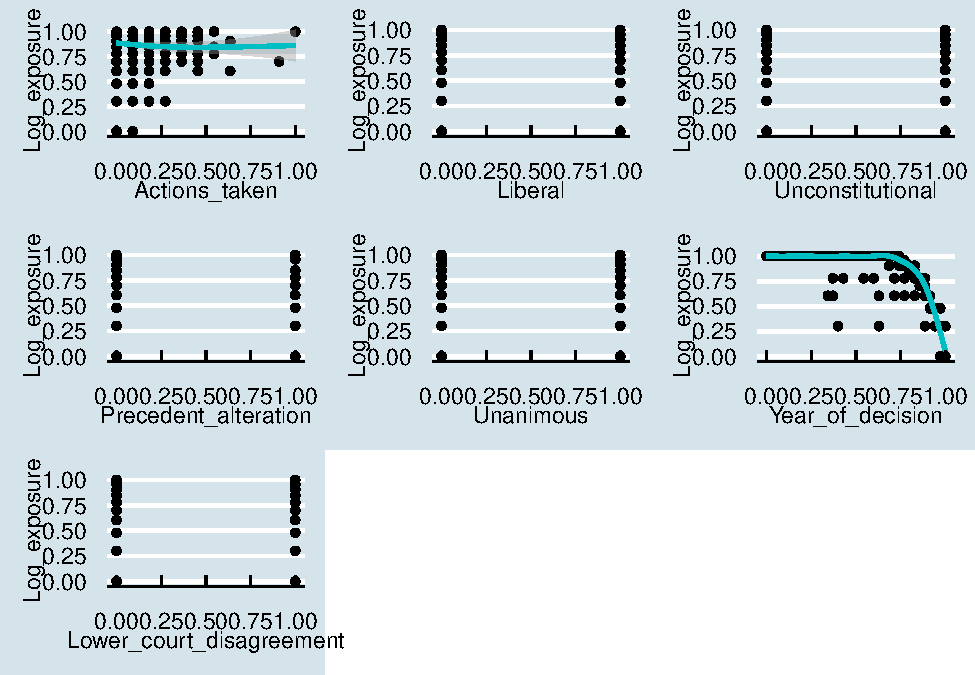
\includegraphics[width=0.8\linewidth]{anacalt-regresion_files/figure-latex/scat_smooth-1} 

}

\caption{Relación de las variables con la salida}\label{fig:scat_smooth}
\end{figure}

Observammos claramente que la variable `Year\_of\_decision' tiene una
relación cuadrática con la variable de output. Por lo que vamos a añadir
una variable polinómica de grado 2 de `Year\_of\_decision'.

\begin{verbatim}
## 
## Call:
## lm(formula = train_lbl ~ Unconstitutional + Actions_taken * Year_of_decision * 
##     Lower_court_disagreement + Year_of_decision * Liberal + I(Year_of_decision^2), 
##     data = train)
## 
## Residuals:
##      Min       1Q   Median       3Q      Max 
## -0.66719 -0.07020 -0.00678  0.08474  0.28094 
## 
## Coefficients:
##                                                           Estimate Std. Error
## (Intercept)                                              0.8177403  0.0093725
## Unconstitutional                                        -0.0033972  0.0076467
## Actions_taken                                           -1.0586195  0.1575175
## Year_of_decision                                         1.4724720  0.0314164
## Lower_court_disagreement                                 0.0193753  0.0109466
## Liberal                                                 -0.0162062  0.0090481
## I(Year_of_decision^2)                                   -1.9205788  0.0273326
## Actions_taken:Year_of_decision                           1.5329778  0.2146916
## Actions_taken:Lower_court_disagreement                   0.9711665  0.4970884
## Year_of_decision:Lower_court_disagreement               -0.0373579  0.0168488
## Year_of_decision:Liberal                                 0.0006344  0.0144260
## Actions_taken:Year_of_decision:Lower_court_disagreement -1.2393915  0.6215945
##                                                         t value Pr(>|t|)    
## (Intercept)                                              87.249  < 2e-16 ***
## Unconstitutional                                         -0.444   0.6569    
## Actions_taken                                            -6.721 2.13e-11 ***
## Year_of_decision                                         46.870  < 2e-16 ***
## Lower_court_disagreement                                  1.770   0.0768 .  
## Liberal                                                  -1.791   0.0734 .  
## I(Year_of_decision^2)                                   -70.267  < 2e-16 ***
## Actions_taken:Year_of_decision                            7.140 1.14e-12 ***
## Actions_taken:Lower_court_disagreement                    1.954   0.0508 .  
## Year_of_decision:Lower_court_disagreement                -2.217   0.0267 *  
## Year_of_decision:Liberal                                  0.044   0.9649    
## Actions_taken:Year_of_decision:Lower_court_disagreement  -1.994   0.0462 *  
## ---
## Signif. codes:  0 '***' 0.001 '**' 0.01 '*' 0.05 '.' 0.1 ' ' 1
## 
## Residual standard error: 0.1121 on 3231 degrees of freedom
## Multiple R-squared:  0.7817, Adjusted R-squared:  0.781 
## F-statistic:  1052 on 11 and 3231 DF,  p-value: < 2.2e-16
\end{verbatim}

Observamos que hemos pegado un salto significativo en el R\^{}2
ajustado, pasando de 0.4464 a 0.781. Por lo que vamos a dejar el modelo
con la variable polinómica. Tras esto, podemos probar a eliminar algunas
de las variables que no son significativas ya que esta adición de la
variable polinómica ha podido hacer que algunas variables que antes sí
eran significativas ahora ya no. Es el caso de la interacción de
`Year\_of\_decision' y `Liberal'. Al eliminarla el R\^{}2 ajustado se
mantiene igual, por lo que la eliminamos. Además, la variable
`Unconstitutional' ya no es significativa, por lo que probamos a
eliminarla también

\begin{verbatim}
## 
## Call:
## lm(formula = train_lbl ~ Liberal + Actions_taken * Year_of_decision * 
##     Lower_court_disagreement + I(Year_of_decision^2), data = train)
## 
## Residuals:
##      Min       1Q   Median       3Q      Max 
## -0.66722 -0.07302 -0.00661  0.08465  0.28080 
## 
## Coefficients:
##                                                          Estimate Std. Error
## (Intercept)                                              0.817887   0.007750
## Liberal                                                 -0.016344   0.004021
## Actions_taken                                           -1.058360   0.157464
## Year_of_decision                                         1.471208   0.029418
## Lower_court_disagreement                                 0.019350   0.010943
## I(Year_of_decision^2)                                   -1.919218   0.027017
## Actions_taken:Year_of_decision                           1.533748   0.214590
## Actions_taken:Lower_court_disagreement                   0.975282   0.496850
## Year_of_decision:Lower_court_disagreement               -0.037395   0.016844
## Actions_taken:Year_of_decision:Lower_court_disagreement -1.244957   0.621225
##                                                         t value Pr(>|t|)    
## (Intercept)                                             105.540  < 2e-16 ***
## Liberal                                                  -4.065 4.92e-05 ***
## Actions_taken                                            -6.721 2.12e-11 ***
## Year_of_decision                                         50.010  < 2e-16 ***
## Lower_court_disagreement                                  1.768   0.0771 .  
## I(Year_of_decision^2)                                   -71.037  < 2e-16 ***
## Actions_taken:Year_of_decision                            7.147 1.09e-12 ***
## Actions_taken:Lower_court_disagreement                    1.963   0.0497 *  
## Year_of_decision:Lower_court_disagreement                -2.220   0.0265 *  
## Actions_taken:Year_of_decision:Lower_court_disagreement  -2.004   0.0451 *  
## ---
## Signif. codes:  0 '***' 0.001 '**' 0.01 '*' 0.05 '.' 0.1 ' ' 1
## 
## Residual standard error: 0.1121 on 3233 degrees of freedom
## Multiple R-squared:  0.7817, Adjusted R-squared:  0.7811 
## F-statistic:  1286 on 9 and 3233 DF,  p-value: < 2.2e-16
\end{verbatim}

Vemos que nuestro R\^{}2 ajustado ha incrementado casi
imperceptiblemente, pero este es más sencillo de interpretar. Probamos
también a eliminar la interacción a 3 niveles, ya que es la menos
significativa, y vemos que el R\^{}2 ajustado baja, por lo que la
dejamos. A continuación, ya que hemos añadido una
Year\_of\_decision\^{}2 y ha funcionado tan bien, probamos a añadir
Year\_of\_decision\^{}3.

\begin{verbatim}
## 
## Call:
## lm(formula = train_lbl ~ Liberal + Actions_taken * Year_of_decision * 
##     Lower_court_disagreement + I(Year_of_decision^2) + I(Year_of_decision^3), 
##     data = train)
## 
## Residuals:
##      Min       1Q   Median       3Q      Max 
## -0.70946 -0.04056  0.01221  0.04898  0.16210 
## 
## Coefficients:
##                                                          Estimate Std. Error
## (Intercept)                                              1.135067   0.005645
## Liberal                                                  0.003745   0.002230
## Actions_taken                                           -0.881614   0.086861
## Year_of_decision                                        -1.949215   0.042947
## Lower_court_disagreement                                 0.007733   0.006036
## I(Year_of_decision^2)                                    6.069486   0.094062
## I(Year_of_decision^3)                                   -5.091218   0.059189
## Actions_taken:Year_of_decision                           1.104623   0.118444
## Actions_taken:Lower_court_disagreement                   0.520234   0.274048
## Year_of_decision:Lower_court_disagreement               -0.013596   0.009293
## Actions_taken:Year_of_decision:Lower_court_disagreement -0.619932   0.342662
##                                                         t value Pr(>|t|)    
## (Intercept)                                             201.090   <2e-16 ***
## Liberal                                                   1.680   0.0931 .  
## Actions_taken                                           -10.150   <2e-16 ***
## Year_of_decision                                        -45.387   <2e-16 ***
## Lower_court_disagreement                                  1.281   0.2003    
## I(Year_of_decision^2)                                    64.527   <2e-16 ***
## I(Year_of_decision^3)                                   -86.016   <2e-16 ***
## Actions_taken:Year_of_decision                            9.326   <2e-16 ***
## Actions_taken:Lower_court_disagreement                    1.898   0.0577 .  
## Year_of_decision:Lower_court_disagreement                -1.463   0.1436    
## Actions_taken:Year_of_decision:Lower_court_disagreement  -1.809   0.0705 .  
## ---
## Signif. codes:  0 '***' 0.001 '**' 0.01 '*' 0.05 '.' 0.1 ' ' 1
## 
## Residual standard error: 0.06179 on 3232 degrees of freedom
## Multiple R-squared:  0.9336, Adjusted R-squared:  0.9334 
## F-statistic:  4546 on 10 and 3232 DF,  p-value: < 2.2e-16
\end{verbatim}

Vemos que sorprendentemente, hay un salto significativo a un R\^{}2
ajustado de 0.9334. Vemos que nuestra interacción ``estrella'' ya no
parece ser tan significativa, por lo que probamos a eliminarla y el
R\^{}2 ajustado se mantiene. Tras esto vemos que además las
interacciones de 2 niveles de Actions\_taken con
Lower\_court\_disagreement y Year\_of\_decision con
Lower\_court\_disagreement ya no son significativas, por lo que las
eliminamos también.

\begin{verbatim}
## 
## Call:
## lm(formula = train_lbl ~ Liberal + Lower_court_disagreement + 
##     Actions_taken * Year_of_decision + I(Year_of_decision^2) + 
##     I(Year_of_decision^3), data = train)
## 
## Residuals:
##      Min       1Q   Median       3Q      Max 
## -0.71123 -0.04089  0.01117  0.04807  0.15434 
## 
## Coefficients:
##                                  Estimate Std. Error t value Pr(>|t|)    
## (Intercept)                     1.1364096  0.0055573 204.491   <2e-16 ***
## Liberal                         0.0038609  0.0022274   1.733   0.0831 .  
## Lower_court_disagreement        0.0001877  0.0026076   0.072   0.9426    
## Actions_taken                  -0.8359121  0.0816293 -10.240   <2e-16 ***
## Year_of_decision               -1.9527494  0.0429177 -45.500   <2e-16 ***
## I(Year_of_decision^2)           6.0744191  0.0940729  64.571   <2e-16 ***
## I(Year_of_decision^3)          -5.0961926  0.0591704 -86.127   <2e-16 ***
## Actions_taken:Year_of_decision  1.0488923  0.1089605   9.626   <2e-16 ***
## ---
## Signif. codes:  0 '***' 0.001 '**' 0.01 '*' 0.05 '.' 0.1 ' ' 1
## 
## Residual standard error: 0.06183 on 3235 degrees of freedom
## Multiple R-squared:  0.9335, Adjusted R-squared:  0.9334 
## F-statistic:  6487 on 7 and 3235 DF,  p-value: < 2.2e-16
\end{verbatim}

Se mantiene el R\^{}2 ajustado, y vemos que la variable
Lower\_court\_disagreement ya no es significativa, eso explica por que
las interacciones tampoco lo eran, por lo que la eliminamos.

\begin{verbatim}
## 
## Call:
## lm(formula = train_lbl ~ Liberal + Actions_taken * Year_of_decision + 
##     I(Year_of_decision^2) + I(Year_of_decision^3), data = train)
## 
## Residuals:
##      Min       1Q   Median       3Q      Max 
## -0.71127 -0.04093  0.01113  0.04804  0.15433 
## 
## Coefficients:
##                                 Estimate Std. Error t value Pr(>|t|)    
## (Intercept)                     1.136444   0.005536 205.284   <2e-16 ***
## Liberal                         0.003862   0.002227   1.734    0.083 .  
## Actions_taken                  -0.836035   0.081599 -10.246   <2e-16 ***
## Year_of_decision               -1.952743   0.042911 -45.507   <2e-16 ***
## I(Year_of_decision^2)           6.074394   0.094058  64.581   <2e-16 ***
## I(Year_of_decision^3)          -5.096144   0.059158 -86.145   <2e-16 ***
## Actions_taken:Year_of_decision  1.049026   0.108928   9.630   <2e-16 ***
## ---
## Signif. codes:  0 '***' 0.001 '**' 0.01 '*' 0.05 '.' 0.1 ' ' 1
## 
## Residual standard error: 0.06182 on 3236 degrees of freedom
## Multiple R-squared:  0.9335, Adjusted R-squared:  0.9334 
## F-statistic:  7571 on 6 and 3236 DF,  p-value: < 2.2e-16
\end{verbatim}

Se mantiene el R\^{}2 ajustado y vemos como parece que la variable
Liberal también ha dejado de ser significativa, por lo que la
eliminamos.

\begin{verbatim}
## 
## Call:
## lm(formula = train_lbl ~ Actions_taken * Year_of_decision + I(Year_of_decision^2) + 
##     I(Year_of_decision^3), data = train)
## 
## Residuals:
##      Min       1Q   Median       3Q      Max 
## -0.71318 -0.03920  0.00954  0.04965  0.15162 
## 
## Coefficients:
##                                 Estimate Std. Error t value Pr(>|t|)    
## (Intercept)                     1.138531   0.005405 210.637   <2e-16 ***
## Actions_taken                  -0.835528   0.081624 -10.236   <2e-16 ***
## Year_of_decision               -1.947144   0.042803 -45.491   <2e-16 ***
## I(Year_of_decision^2)           6.057918   0.093606  64.717   <2e-16 ***
## I(Year_of_decision^3)          -5.085534   0.058858 -86.403   <2e-16 ***
## Actions_taken:Year_of_decision  1.049787   0.108961   9.635   <2e-16 ***
## ---
## Signif. codes:  0 '***' 0.001 '**' 0.01 '*' 0.05 '.' 0.1 ' ' 1
## 
## Residual standard error: 0.06183 on 3237 degrees of freedom
## Multiple R-squared:  0.9334, Adjusted R-squared:  0.9333 
## F-statistic:  9079 on 5 and 3237 DF,  p-value: < 2.2e-16
\end{verbatim}

Vemos que el modelo ha pasado de un R\^{}2 ajustado de 0.9334 a 0.9333
por lo que, al ser un cambio tan pequeño y dado que el modelo pasa a ser
más interpretable, vamos a dejar este modelo. Siguiendo con la misma
lógica hasta ahora, probaremos a añaadir Year\_of\_decision\^{}4.

\begin{verbatim}
## 
## Call:
## lm(formula = train_lbl ~ Actions_taken * Year_of_decision + I(Year_of_decision^2) + 
##     I(Year_of_decision^3) + I(Year_of_decision^4), data = train)
## 
## Residuals:
##      Min       1Q   Median       3Q      Max 
## -0.68369 -0.01281  0.00122  0.01640  0.23451 
## 
## Coefficients:
##                                  Estimate Std. Error t value Pr(>|t|)    
## (Intercept)                      0.941361   0.004426 212.680   <2e-16 ***
## Actions_taken                   -0.605521   0.051625 -11.729   <2e-16 ***
## Year_of_decision                 1.403190   0.055007  25.509   <2e-16 ***
## I(Year_of_decision^2)           -7.934629   0.208656 -38.027   <2e-16 ***
## I(Year_of_decision^3)           15.698688   0.299561  52.406   <2e-16 ***
## I(Year_of_decision^4)          -10.047861   0.143701 -69.922   <2e-16 ***
## Actions_taken:Year_of_decision   0.657709   0.069003   9.532   <2e-16 ***
## ---
## Signif. codes:  0 '***' 0.001 '**' 0.01 '*' 0.05 '.' 0.1 ' ' 1
## 
## Residual standard error: 0.03903 on 3236 degrees of freedom
## Multiple R-squared:  0.9735, Adjusted R-squared:  0.9734 
## F-statistic: 1.981e+04 on 6 and 3236 DF,  p-value: < 2.2e-16
\end{verbatim}

Vemos que el R\^{}2 ajustado ha pasado de 0.9333 a 0.9734, por lo que
conseguimos otro salto. Probamos por lo tanto con
Year\_of\_decision\^{}5.

\begin{verbatim}
## 
## Call:
## lm(formula = train_lbl ~ Actions_taken * Year_of_decision + I(Year_of_decision^2) + 
##     I(Year_of_decision^3) + I(Year_of_decision^4) + I(Year_of_decision^5), 
##     data = train)
## 
## Residuals:
##      Min       1Q   Median       3Q      Max 
## -0.66620 -0.00303  0.00019  0.00269  0.26726 
## 
## Coefficients:
##                                  Estimate Std. Error t value Pr(>|t|)    
## (Intercept)                      1.012997   0.004953 204.535  < 2e-16 ***
## Actions_taken                   -0.623318   0.047236 -13.196  < 2e-16 ***
## Year_of_decision                -0.433806   0.088766  -4.887 1.07e-06 ***
## I(Year_of_decision^2)            4.010880   0.512383   7.828 6.67e-15 ***
## I(Year_of_decision^3)          -14.633710   1.238105 -11.819  < 2e-16 ***
## I(Year_of_decision^4)           22.834309   1.315471  17.358  < 2e-16 ***
## I(Year_of_decision^5)          -12.762099   0.507999 -25.122  < 2e-16 ***
## Actions_taken:Year_of_decision   0.669193   0.063131  10.600  < 2e-16 ***
## ---
## Signif. codes:  0 '***' 0.001 '**' 0.01 '*' 0.05 '.' 0.1 ' ' 1
## 
## Residual standard error: 0.03571 on 3235 degrees of freedom
## Multiple R-squared:  0.9778, Adjusted R-squared:  0.9778 
## F-statistic: 2.037e+04 on 7 and 3235 DF,  p-value: < 2.2e-16
\end{verbatim}

Vemos que incrementar el exponente sigue mejorando el modelo, llegando a
R\^{}2 de 0.9778 por lo que probamos con Year\_of\_decision\^{}6 y vemos
que el R\^{}2 ajustado ha pasado de 0.9778 a 0.9779 por lo que no parece
que tenga sentido seguir incrementando el exponente y nos quedamos con
el modelo anterior.

Hemos conseguido un modelo que alcanza un R\^{}2 ajustado de 0.9778. Lo
que significa que el 97.78\% de la variabilidad de la variable
Log\_exposure es explicada por nuestro modelo. Observamos como se ajusta
este modelo a los datos en la Figura \ref{fig:model_pol}. Calculamos
también el MSE (Mean Squared Error) con el conjunto de test.

\begin{verbatim}
## [1] "MSE: 0.0011"
\end{verbatim}

\begin{figure}

{\centering 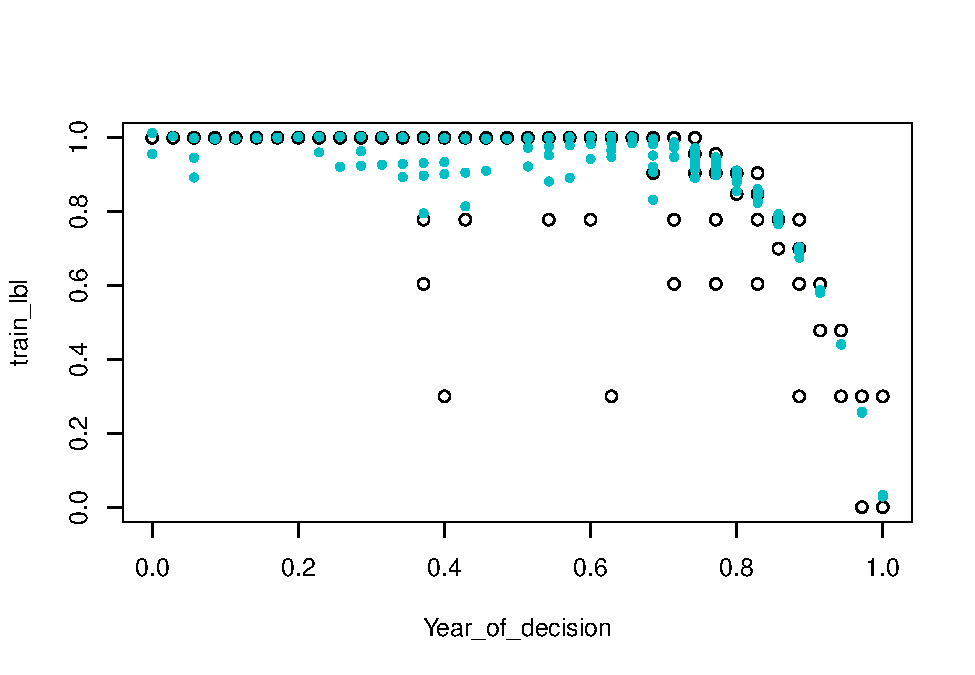
\includegraphics[width=0.75\linewidth]{anacalt-regresion_files/figure-latex/model_pol-1} 

}

\caption{Ajuste del modelo polinómico}\label{fig:model_pol}
\end{figure}

\hypertarget{validaciuxf3n-cruzada-k-fold-cross-validation}{%
\subsubsection{Validación cruzada (K-fold cross
validation)}\label{validaciuxf3n-cruzada-k-fold-cross-validation}}

Para comprobar que nuestro modelo no está sobreajustado, vamos a
realizar una validación cruzada con las 5 particiones que se indicaron
junto al dataset. Por un lado usando el modelo de todas las variables y
por otro usando el modelo polinómico que hemos obtenido
\texttt{\textquotesingle{}Y\ \textasciitilde{}\ X1*X6\ +\ I(X6\^{}2)\ +\ I(X6\^{}3)\ +\ I(X6\^{}4)\ +\ I(X6\^{}5)\textquotesingle{}}.
Donde podemos observar como el MSE es mucho mejor en nuestro modelo que
en el modelo con todas las variables.

\begin{verbatim}
## [1] "MSE del modelo con todas las variables en train: 0.1699"
\end{verbatim}

\begin{verbatim}
## [1] "MSE del modelo con todas las variables en test: 0.171"
\end{verbatim}

\begin{verbatim}
## [1] "MSE del modelo polinómico en train: 0.007"
\end{verbatim}

\begin{verbatim}
## [1] "MSE del modelo polinómico en test: 0.0074"
\end{verbatim}

\hypertarget{regresiuxf3n-usando-k-nearest-neighbors}{%
\subsection{Regresión usando K-Nearest
Neighbors}\label{regresiuxf3n-usando-k-nearest-neighbors}}

Vamos a probar a realizar la regresión usando el algoritmo K-Nearest
Neighbors. Para ello vamos a usar la librería \texttt{kknn}. Primero
vamos a probar a usar todas las variables y luego vamos a probar a usar
las variables más significativas que hemos obtenido con la regresión
lineal.

\hypertarget{modelo-con-todas-las-variables}{%
\subsubsection{Modelo con todas las
variables}\label{modelo-con-todas-las-variables}}

Probamos primeramente con todas las variables y con \texttt{k\ =\ 7} que
es el valor por defecto.

\begin{Shaded}
\begin{Highlighting}[]
\NormalTok{modelknn }\OtherTok{\textless{}{-}} \FunctionTok{kknn}\NormalTok{(train\_lbl }\SpecialCharTok{\textasciitilde{}}\NormalTok{ ., train, test) }\CommentTok{\# Por defecto k = 7}
\end{Highlighting}
\end{Shaded}

\begin{verbatim}
## [1] "MSE frente a test: 0.0022"
\end{verbatim}

Si nos fijamos en el MSE el modelo de KNN parece prometedor, ya que
parece tener menos error que el modelo linear de regresión. Probamos a
ajustar el valor de K para ver si mejora el modelo, podemos ver el
rendimiento en la Figura \ref{fig:k_mse}.

\begin{figure}

{\centering 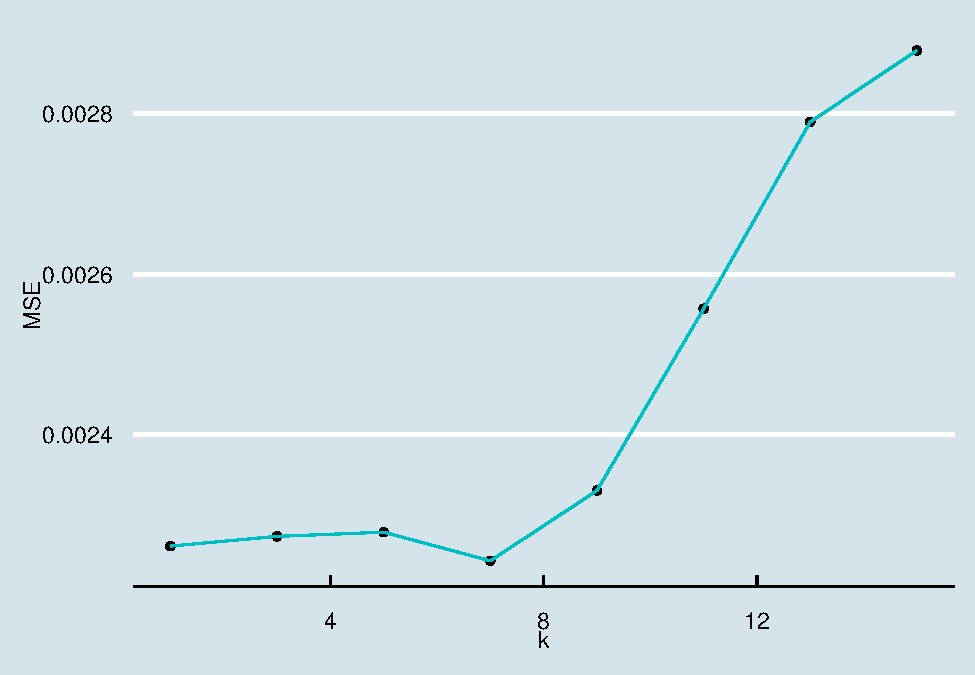
\includegraphics[width=0.5\linewidth]{anacalt-regresion_files/figure-latex/k_mse-1} 

}

\caption{Ajuste del valor de K frente MSE}\label{fig:k_mse}
\end{figure}

Podemos observar como el modelo con \texttt{k=7} es el que mejor
resultado tiene. Ploteamos el modelo para ver cómo se ajusta a los datos
(Figura \ref{fig:model_knn}).

\begin{figure}

{\centering 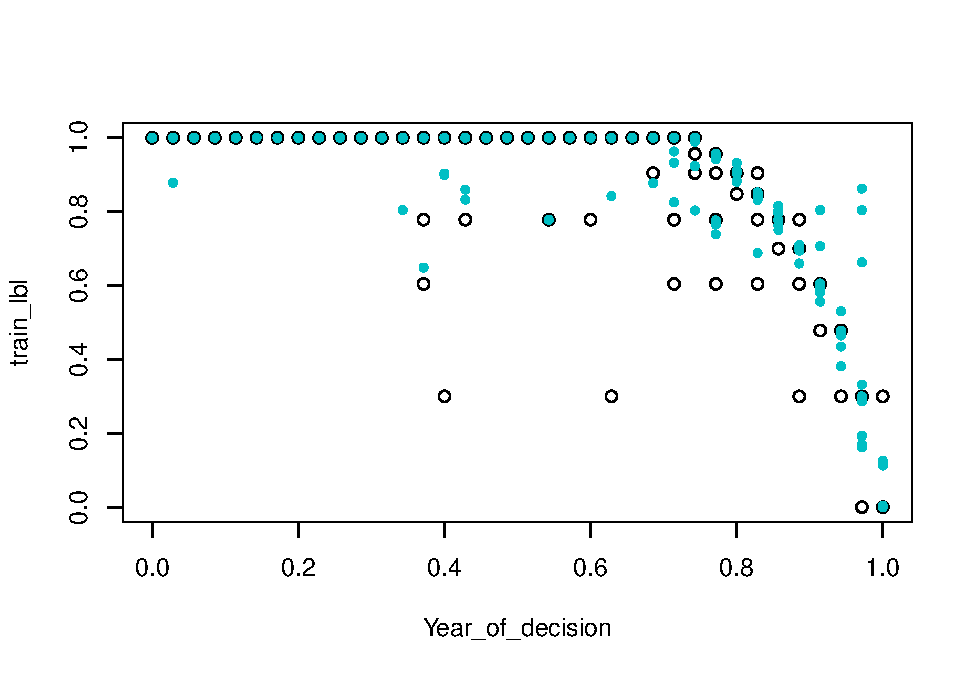
\includegraphics[width=0.5\linewidth]{anacalt-regresion_files/figure-latex/model_knn-1} 

}

\caption{Modelo KNN con k=7}\label{fig:model_knn}
\end{figure}

\hypertarget{modelo-con-la-fuxf3rmula-usada-en-regresiuxf3n-lineal}{%
\subsubsection{Modelo con la fórmula usada en regresión
lineal}\label{modelo-con-la-fuxf3rmula-usada-en-regresiuxf3n-lineal}}

Podemos probar a ver si usando la misma fórmula que con la regresión
lineal
(\texttt{Log\_exposure\ \textasciitilde{}\ Actions\_taken*Year\_of\_decision\ +\ I(Year\_of\_decision\^{}2)\ +\ I(Year\_of\_decision\^{}3)\ +\ I(Year\_of\_decision\^{}4)\ +\ I(Year\_of\_decision\^{}5)})
mejoramos el modelo. Usamos \texttt{k\ =\ 7} que es el valor por
defecto.

\begin{verbatim}
## [1] "MSE frente a test: 0.001"
\end{verbatim}

Vemos que el error ha disminuido por lo que incluso en KNN parece que la
fórmula polinómica tiene bastante éxito. Ploteamos el modelo para ver
cómo se ajusta a los datos (Figura \ref{fig:model_knn_2}).

\begin{figure}

{\centering 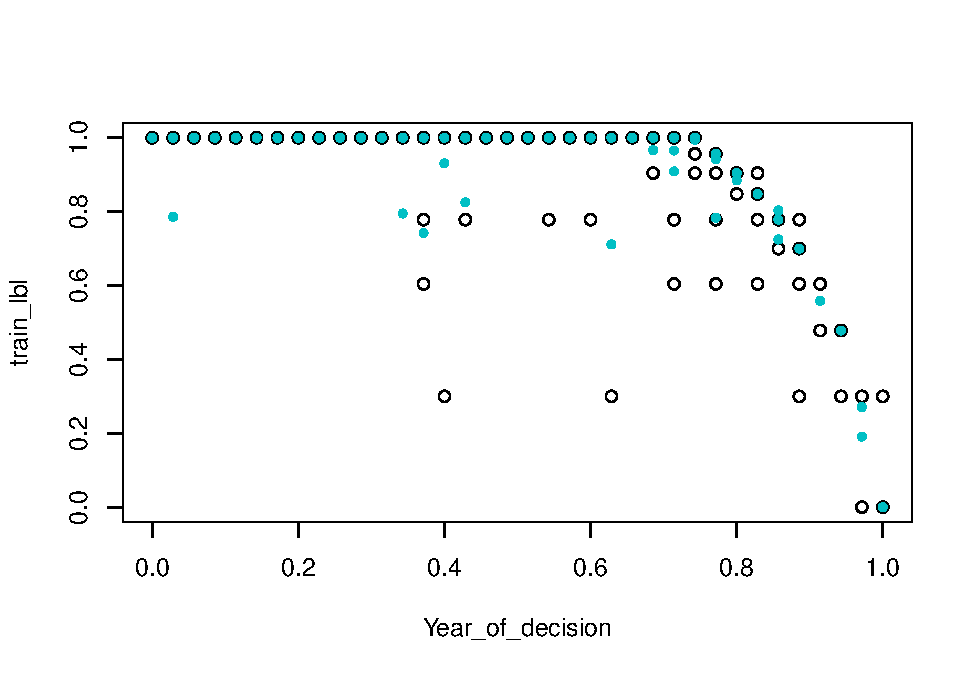
\includegraphics[width=0.5\linewidth]{anacalt-regresion_files/figure-latex/model_knn_2-1} 

}

\caption{Modelo KNN con k=7 y fórmula customizada}\label{fig:model_knn_2}
\end{figure}

\hypertarget{validaciuxf3n-cruzada-k-fold-cross-validation-1}{%
\subsubsection{Validación cruzada (K-fold cross
validation)}\label{validaciuxf3n-cruzada-k-fold-cross-validation-1}}

Para asegurarnos de que esta disminución del error no es casualidad o un
sobreajuste, vamos a realizar una validación cruzada.

\begin{verbatim}
## [1] "MSE del modelo con todas las variables en train: 0.0063"
\end{verbatim}

\begin{verbatim}
## [1] "MSE del modelo con todas las variables en test: 0.0115"
\end{verbatim}

\begin{verbatim}
## [1] "MSE del modelo con la fórmula polinómica en train: 0.0043"
\end{verbatim}

\begin{verbatim}
## [1] "MSE del modelo con la fórmula polinómica en test: 0.0073"
\end{verbatim}

Podemos observar como KNN suele sobreajustar, podemos intuirlo ya que
tiene casi el doble de error en test que en train. Aun así, los datos de
error son menores en general que los de regresión lineal.

\hypertarget{comparaciuxf3n-de-los-modelos}{%
\subsection{Comparación de los
modelos}\label{comparaciuxf3n-de-los-modelos}}

Como paso final, vamos a comparar los modelos de regresión lineal y KNN
con M5P. Los resultados de los correspondientes MSE de los modelos con
todas las variables los tenemos almacenados en CSV's. Los cargamos y los
comparamos.

\begin{verbatim}
## [1] "Summary de los datos de train:"
\end{verbatim}

\begin{verbatim}
##       X              out_train_lm       out_train_kknn      out_train_m5p      
##  Length:18          Min.   :0.000e+00   Min.   :0.000e+00   Min.   :0.000e+00  
##  Class :character   1st Qu.:0.000e+00   1st Qu.:0.000e+00   1st Qu.:0.000e+00  
##  Mode  :character   Median :5.000e+00   Median :2.000e+00   Median :3.000e+00  
##                     Mean   :3.827e+08   Mean   :1.159e+08   Mean   :1.943e+08  
##                     3rd Qu.:8.300e+01   3rd Qu.:2.200e+01   3rd Qu.:2.400e+01  
##                     Max.   :4.826e+09   Max.   :1.561e+09   Max.   :2.559e+09
\end{verbatim}

\begin{verbatim}
## [1] "Summary de los datos de test:"
\end{verbatim}

\begin{verbatim}
##       X              out_test_lm        out_test_kknn        out_test_m5p      
##  Length:18          Min.   :0.000e+00   Min.   :0.000e+00   Min.   :0.000e+00  
##  Class :character   1st Qu.:0.000e+00   1st Qu.:0.000e+00   1st Qu.:0.000e+00  
##  Mode  :character   Median :5.000e+00   Median :6.000e+00   Median :3.000e+00  
##                     Mean   :3.843e+08   Mean   :2.929e+08   Mean   :2.480e+08  
##                     3rd Qu.:8.500e+01   3rd Qu.:5.300e+01   3rd Qu.:3.100e+01  
##                     Max.   :4.844e+09   Max.   :3.846e+09   Max.   :3.158e+09
\end{verbatim}

Para visualizarlo de mejor manera ploteamos los diferentes MSE para
nuestro dataset (Figura \ref{fig:mse_comp})

\begin{figure}

{\centering 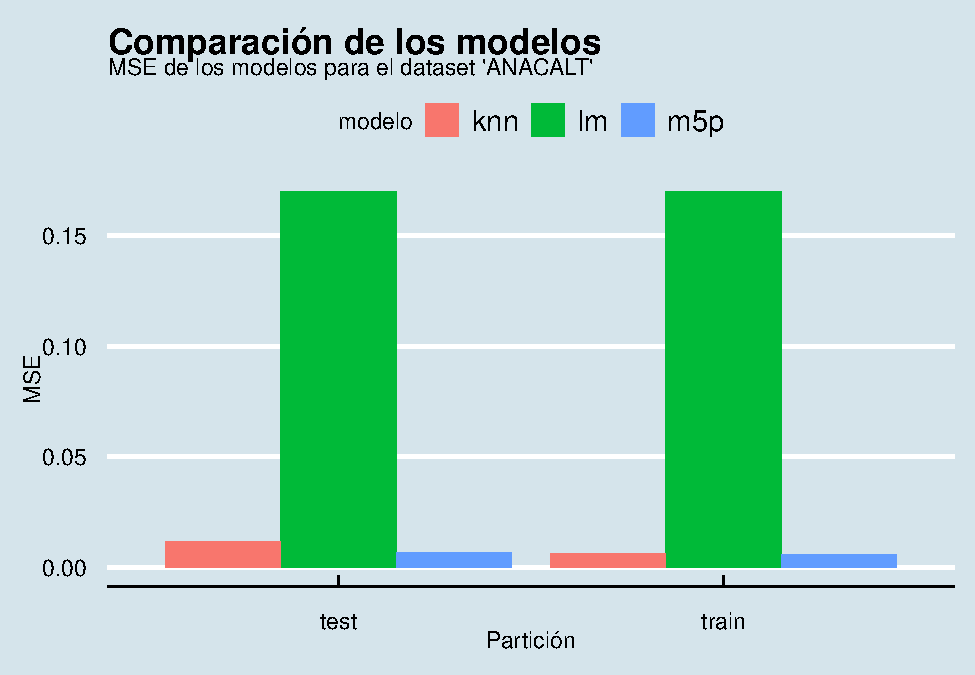
\includegraphics[width=0.75\linewidth]{anacalt-regresion_files/figure-latex/mse_comp-1} 

}

\caption{Comparación de los MSE de los modelos de regresión lineal, KNN y M5P para el dataset ANACALT}\label{fig:mse_comp}
\end{figure}

\begin{verbatim}
## List of 2
##  $ plot.title   :List of 11
##   ..$ family       : NULL
##   ..$ face         : NULL
##   ..$ colour       : NULL
##   ..$ size         : NULL
##   ..$ hjust        : num 0.5
##   ..$ vjust        : NULL
##   ..$ angle        : NULL
##   ..$ lineheight   : NULL
##   ..$ margin       : NULL
##   ..$ debug        : NULL
##   ..$ inherit.blank: logi FALSE
##   ..- attr(*, "class")= chr [1:2] "element_text" "element"
##  $ plot.subtitle:List of 11
##   ..$ family       : NULL
##   ..$ face         : NULL
##   ..$ colour       : NULL
##   ..$ size         : NULL
##   ..$ hjust        : num 0.5
##   ..$ vjust        : NULL
##   ..$ angle        : NULL
##   ..$ lineheight   : NULL
##   ..$ margin       : NULL
##   ..$ debug        : NULL
##   ..$ inherit.blank: logi FALSE
##   ..- attr(*, "class")= chr [1:2] "element_text" "element"
##  - attr(*, "class")= chr [1:2] "theme" "gg"
##  - attr(*, "complete")= logi FALSE
##  - attr(*, "validate")= logi TRUE
\end{verbatim}

De primeras, podemos observar como LM tiene bastante peor rendimiento en
los modelos de todas las variables. Para hacer una comparación rigurosa,
realizamos un test de Friedman.

\begin{verbatim}
## 
##  Friedman rank sum test
## 
## data:  .
## Friedman chi-squared = 8.4444, df = 2, p-value = 0.01467
\end{verbatim}

Como el p-valor es menor que 0.05, podemos rechazar la hipótesis nula de
que los modelos tienen el mismo rendimiento. Para saber cuáles son los
modelos que tienen un rendimiento significativamente diferente,
realizamos una comparación a pares con el post hoc de Holm.

\begin{verbatim}
## 
##  Pairwise comparisons using Wilcoxon signed rank exact test 
## 
## data:  al_matrix and groups 
## 
##   1     2    
## 2 0.580 -    
## 3 0.081 0.108
## 
## P value adjustment method: holm
\end{verbatim}

Vemos que el p-valor entre el primer y el segundo algoritmo es 0.580,
por lo que hay diferencias significativas entre ellos. O sea, parece
haber diferencias significativas entre LM y KNN. El p-valor entre el
primer y el tercer algoritmo es 0.108, por lo que también hay
diferencias significativas entre ellos. O sea, parece haber diferencias
significativas entre LM y M5'. Y si comparamos el segundo y el tercer
algoritmo, el p-valor es 0.108, por lo que también hay diferencias
significativas entre ellos. O sea, parece haber diferencias
significativas entre KNN y M5'. Por lo tanto, hay diferencias
significativas entre todos los algoritmos y dado que M5' es el que
consigue el p-valor más pequeño, podemos decir que es el mejor
algoritmo.

\hypertarget{anexo-cuxf3digo-de-la-pruxe1ctica}{%
\section{Anexo : Código de la
práctica}\label{anexo-cuxf3digo-de-la-pruxe1ctica}}

Dado que esto se ha realizado en un archivo de RMarkdown, se puede ver
el código de la práctica en el archivo \texttt{pima-cladificacion.Rmd}
que se encuentra en el repositorio de GitHub.
\href{https://github.com/DanelArias-Dreyton257/DATCOM-Intro}{Click aquí}

\end{document}
